% interactcadsample.tex
% v1.03 - April 2017

\documentclass[]{interact}

\usepackage{epstopdf}% To incorporate .eps illustrations using PDFLaTeX, etc.
\usepackage{subfigure}% Support for small, `sub' figures and tables
%\usepackage[nolists,tablesfirst]{endfloat}% To `separate' figures and tables from text if required

\usepackage{natbib}% Citation support using natbib.sty
\bibpunct[, ]{(}{)}{;}{a}{}{,}% Citation support using natbib.sty
\renewcommand\bibfont{\fontsize{10}{12}\selectfont}% Bibliography support using natbib.sty

\theoremstyle{plain}% Theorem-like structures provided by amsthm.sty
\newtheorem{theorem}{Theorem}[section]
\newtheorem{lemma}[theorem]{Lemma}
\newtheorem{corollary}[theorem]{Corollary}
\newtheorem{proposition}[theorem]{Proposition}

\theoremstyle{definition}
\newtheorem{definition}[theorem]{Definition}
\newtheorem{example}[theorem]{Example}

\theoremstyle{remark}
\newtheorem{remark}{Remark}
\newtheorem{notation}{Notation}


% tightlist command for lists without linebreak
\providecommand{\tightlist}{%
  \setlength{\itemsep}{0pt}\setlength{\parskip}{0pt}}



\usepackage{hyperref}
\usepackage[utf8]{inputenc}
\def\tightlist{}
\usepackage{setspace}\doublespacing
\usepackage{graphicx}
\usepackage{nicematrix}
\NiceMatrixOptions{code-for-first-row = \color{red} ,code-for-last-row = \color{red} ,code-for-first-col = \color{blue} ,code-for-last-col = \color{blue}}


\begin{document}


\articletype{Short Technical Note}

\title{New and simplified manual controls for projection and slice
tours, with application to exploring classification boundaries in high
dimensions}


\author{\name{Ursula Laa$^{a}$, Alex Aumann$^{b}$, Dianne
Cook$^{c}$, German Valencia$^{b}$}
\affil{$^{a}$Institute of Statistics, University of Natural Resources
and Life Sciences, Vienna; $^{b}$School of Physics and Astronomy, Monash
University; $^{c}$Department of Econometrics and Business Statistics,
Monash University}
}

\thanks{CONTACT Ursula
Laa. Email: \href{mailto:ursula.laa@boku.ac.at}{\nolinkurl{ursula.laa@boku.ac.at}}, Alex
Aumann. Email: \href{mailto:aaum0002@student.monash.edu}{\nolinkurl{aaum0002@student.monash.edu}}, Dianne
Cook. Email: \href{mailto:dicook@monash.edu}{\nolinkurl{dicook@monash.edu}}, German
Valencia. Email: \href{mailto:german.valencia@monash.edu}{\nolinkurl{german.valencia@monash.edu}}}

\maketitle

\begin{abstract}
This paper describes new user controls for examining high-dimensional
data using low-dimensional linear projections and slices. A user can
interactively change the contribution of a given variable to a
low-dimensional projection, which is useful for exploring the
sensitivity of structure to particular variables. The user can also
interactively shift the center of a slice, for example, to explore how
structure changes in local subspaces. The Mathematica package as well as
example notebooks are provided, which contain functions enabling the
user to experiment with these new manual controls, with one specifically
for exploring regions and boundaries produced by classification models.
The advantage of Mathematica is its linear algebra capabilities and
interactive cursor location controls. Some limited implementation has
also been made available in the R package \tt{tourr}. 
\end{abstract}

\begin{keywords}
data visualisation; grand tour; statistical computing; statistical
graphics; multivariate data; dynamic graphics
\end{keywords}

\hypertarget{introduction}{%
\section{Introduction}\label{introduction}}

From a statistical perspective 3D is a rare data dimension, so unlike in
most 3D rotation computer graphics applications,
\textcolor{blue}{methods which work for arbitrary dimensions have more general utility}.
A good approach is to show projections from an arbitrary dimensional
space to create dynamic data visualizations called \emph{tours}. Tours
involve views of high-dimensional data with low-dimensional projections.
In his original paper on the grand tour, \citet{As85} provided several
algorithms for tour paths that could theoretically show the viewer the
data \emph{from all sides}.
\textcolor{blue}{(Various videos of tours, e.g.} \citet{dataviewer},
\citet{gt-pp-video}, on the \citet{ASA22},
\textcolor{blue}{illustrate this concept.)} Prior to Asimov's work,
there were numerous preparatory developments including \citet{tukey}'s
PRIM-9. PRIM-9 had user-controlled rotations on coordinate axes,
allowing one to manually tour through low-dimensional projections. (A
video \citep{PRIM9-video} illustrating the capabilities is available
through \textcolor{blue}{the} video library of \citet{ASA22}.) Steering
through all possible projections is impossible, unlike Asimov's tours
which allow one to quickly see many, many different projections. After
Asimov, there have been many tour developments, which are summarized in
\citet{lee2021}.

One such direction of work develops the ideas from PRIM-9, to provide
manual control of a tour. \citet{cook_manual_1997} describe controls for
1D (or 2D) projections, respectively in a 2D (or 3D) manipulation space,
allowing the user to select any variable axis, and rotate it into, out
of, or around the projection through horizontal, vertical, oblique,
radial or angular changes in value. \citet{spyrison_spinifex_2020}
refined this algorithm and implemented it to generate radial tour
animation sequences.

Manual controls are especially useful for assessing the sensitivity of
structure to particular elements of the projection. There are many
places where it is useful. In exploratory data analysis, where one sees
clusters in a projection, one may ask whether some variables can be
removed from the projection without affecting the clustering. For
interpreting models, one can reduce or increase a variable's
contribution, to examine the variable importance. Having the user
interact with a projection is extremely valuable for understanding
high-dimensional data. However, these algorithms have two problems: (1)
the pre-processing of creating a manipulation space overly complicates
the algorithm, and (2) extending to higher dimensional control is
difficult.

Another potentially useful manual control is to allow the user to choose
the position of the center of a slice. The slice tour was introduced in
\citet{slicetour}. It operates by converting the projection plane into a
slice, by removing or de-emphasizing points that are further than a
fixed orthogonal distance from the plane. The projection plane is
usually thought of as passing through the center of the data. Manual
control would allow the user to change the position of the center point,
by shifting it along a coordinate axis, while keeping the orientation of
the projection plane fixed. The purpose would be to explore how or if
the shape of the data, in the space orthogonal to the projection,
changes as one gets away from the center. It would also allow the user
to interactively decide on the thickness of the slice.

This paper explains the new manual controls for projection and slice
tours. The next section describes the new algorithm for manual control,
for both projections and slices. The use of these methods is illustrated
to compare and contrast boundaries constructed by different classifiers.
The software section describes a Mathematica \citep{Mathematica} package
that is used for the application and describes the interactive
environment that would be desirable within R \citep{rref} as new
technology becomes available. The paper is accompanied by an appendix
with more details and adjustments to the manual controls, and three
Mathematica notebooks that can be used to reproduce the applications.

\hypertarget{sec:method}{%
\section{How to construct a manual tour}\label{sec:method}}

A manual tour allows the user to alter the coefficients of one (or more)
variables, of \(p\), contributing to a \(d\)-dimensional projection. The
initial ingredients are an orthonormal basis (\(A_{p\times d}\))
defining the projection of the data, and a variable id
(\(m \in \{1, ..., p\}\)) specifying which coefficient will be
\textcolor{blue}{changed: the $m^{th}$ row of $A_{p\times d}$ which we denote by $V_m$.}
A method to update the values of the component of the controlled
variable \(V_m\) is then needed.

\hypertarget{existing-methods}{%
\subsection{Existing methods}\label{existing-methods}}

The methods for updating component values in \citet{cook_manual_1997}
(and utilized in \citet{spyrison_spinifex_2020}) are prescribed
primarily for a 2D projection, to take advantage of (then) newly
developed 3D trackball controls made available for computer gaming. The
first step was to construct a 3D manipulation space from a 2D
projection. In this space, the coefficient of the controlled variable
ranges between -1 and 1. Movements of a cursor are recorded and
converted into changes in the values of \(V_m\) thus changing the
displayed 2D projection. The algorithm also provided constraints to
horizontal, vertical, radial, or angular motions only. The construction
of the manipulation space overly complicates the manual controls,
especially when considering possible techniques that will apply to
arbitrary \(d\).

\hypertarget{a-new-simpler-and-broadly-applicable-approach}{%
\subsection{A new simpler and broadly applicable
approach}\label{a-new-simpler-and-broadly-applicable-approach}}

The new approach emerged from experiments on the tour using linear
algebra capabilities, and a relatively new interactive graphics
interface, available in Mathematica. The components corresponding to
\(V_m\) are directly controlled by cursor movement, which updates row
\(m\) of \(A\). The updated matrix is then orthonormalized.

\hypertarget{algorithm}{%
\subsubsection{Algorithm}\label{algorithm}}

\begin{enumerate}
\def\labelenumi{\arabic{enumi}.}
\tightlist
\item
  Provide \(A\), and \(m\). (Note that \(m\) could also be automatically
  chosen as the component that is closest to the cursor position.)
\item
  Change values in row \(m\), for example, if \(d=2\) \[
  A^* = [ \boldsymbol{a}^*_1~\boldsymbol{a}^*_2 ] = \left[ \begin{array}{cc} a_{11} & a_{12}\\
                             \vdots & \vdots \\
                             a^*_{m1} & a^*_{m2}\\
                             \vdots & \vdots \\
                             a_{p1} & a_{p2} 
       \end{array}\right].
  \] \noindent A large change in these values would correspond to making
  a large jump from the current projection. Small changes would
  correspond to tracking a cursor, making small jumps from the current
  projection.
\item
  Orthonormalise \(A^*\), using Gram-Schmidt.

  \begin{enumerate}
  \def\labelenumii{\roman{enumii}.}
  \tightlist
  \item
    Normalise \(\boldsymbol{a}^*_1\) and \(\boldsymbol{a}^*_2\).
  \item
    \(\boldsymbol{a}^*_2 = \boldsymbol{a}^*_2 - (\boldsymbol{a}^*_1\cdot\boldsymbol{a}^*_2)\boldsymbol{a}^*_1\).
  \end{enumerate}
\end{enumerate}

\textcolor{red}{a2 should be normalised after the second step? Fig 1: this is now showing tracking, with the yellow dot moving in each image?}

This algorithm will produce the changes to a projection as illustrated
in Figure \ref{fig:manualsequence}. The controlled variable, \(V_m\),
corresponds to the dark line, and sequential changes to row \(m\) of
\(A\) can be seen to roughly follow a specified position (dot). Changes
in the other components happen as a result of the orthonormalization but
are uncontrolled.

The algorithm will also allow for more than one variable to be
controlled. This is more difficult to implement interactively, but is
easy with scripting, as is available in the R implementation.

\begin{figure}
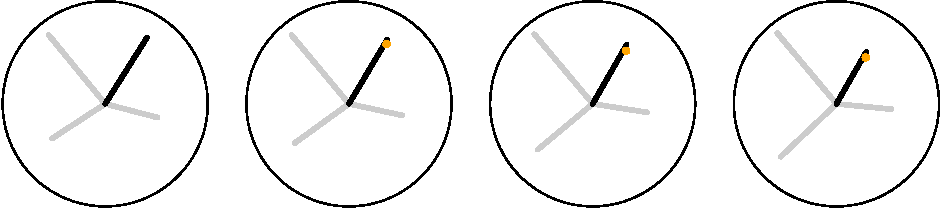
\includegraphics[width=1\linewidth]{paper_files/figure-latex/manualsequence-1} \caption{Sequence of projections where the contribution of one variable is controlled (dark) is changed using unconstrained orthonormalization. The dot indicates the chosen values for the controlled variable, $V_m$. It can be seen that the actual axis does not precisely match the chosen position, but it is close.}\label{fig:manualsequence}
\end{figure}

\hypertarget{refinements-to-enforce-exact-position}{%
\subsection{Refinements to enforce exact
position}\label{refinements-to-enforce-exact-position}}

The problem with the new simple method is that it is not faithful to the
precise values for \(V_m\) because the orthonormalization will change
them. Even though these changes are for the most part imperceptible, one
may wish to avoid them and there are numerous ways that this can be
enforced, a few are detailed in the Appendix. These primarily differ in
how the remaining variables are adjusted during orthonormalization.

\hypertarget{manual-control-for-slices}{%
\subsection{Manual control for slices}\label{manual-control-for-slices}}

To better explore the space we combine the manual controls for the
projection with manual controls for slicing. A slice is a section of the
data that is defined by a projection, a center point that is anchoring
it in the high-dimensional space, and the slice thickness \(h\)
\citep{slicetour}. A data point is inside the slice if its orthogonal
distance from the projection plane (passing through the center point) is
below the thickness \(h\). This orthogonal distance is computed in terms
of the component that is normal on the projection plane. For
\(\mathbf{x}_i\) a \(p\) dimensional data point and \(\mathbf{c}\) the
center point (in the same \(p\) dimensional space) we compute the
orthogonal distance as \begin{equation}
v_i^2 = ||\mathbf{x}_i' - \mathbf{c}'||^2 = \mathbf{x}_i'^2 + \mathbf{c}'^2 - 2 \mathbf{x}_i'\cdot\mathbf{c}' ,
\label{eq:slice}
\end{equation} with
\(\mathbf{c}' = \mathbf{c} - (\mathbf{c}\cdot \mathbf{a}_1) \mathbf{a}_1 - (\mathbf{c}\cdot \mathbf{a}_2 )\mathbf{a}_2\),
\(\mathbf{x}_i' = \mathbf{x}_i - (\mathbf{x}_i\cdot \mathbf{a}_1) \mathbf{a}_1 - (\mathbf{x}_i\cdot \mathbf{a}_2) \mathbf{a}_2\)
and \(\mathbf{a}_k, k=1,2 (=d)\) denoting the columns of the projection
matrix, \(\mathbf{A}=(\mathbf{a}_1, \mathbf{a}_2)\).

\hypertarget{shifting-the-center}{%
\subsubsection{Shifting the center}\label{shifting-the-center}}

A natural starting point is to place \(\mathbf{c}\) in the center of the
data distribution, but shifting it away from the mean can provide
additional insights. In the case of a single orthogonal direction on the
projection plane we can pick a sequence of center points \(\mathbf{c}\)
in steps along that direction to move the slice and fully cover the data
space. This no longer works in higher-dimensional spaces, and we can
think of picking one direction and shifting the slice along the
component orthogonal to the projection plane.

\hypertarget{changing-the-thickness}{%
\subsubsection{Changing the thickness}\label{changing-the-thickness}}

In addition, it is also useful to interactively change the slice
thickness \(h\) (also called the slice radius), in particular, to find
the preferred value for exploring the input data. For guidance the
estimates of the number of points inside the slice as a function of the
original sample size \(N\) and the number of dimensions \(p\) from
\citet{sectionpursuit} can be used: in case of a uniform distribution
inside a sphere of radius \(R\) a slice with thickness \(h\) will
contain \(N_S\) points, with \begin{equation}
N_S(h, p, R, N) = \frac{N}{2} \left(\frac{h}{R}\right)^{p-2} \left(p - (p-2)\left(\frac{h}{R}\right)^{2}\right).
\label{eq:count}
\end{equation}

\hypertarget{sec:implementation}{%
\section{Software}\label{sec:implementation}}

The implementation of the manual tour as suggested here requires the
visualization of the current projection in terms of an axis display (see
Figure \ref{fig:manualsequence} for an example). This display should be
able to track the mouse position and adjust the projection based on the
\textcolor{blue}{user's cursor position}. The user can select one axis
(corresponding to one variable) by clicking on it, and then adjust the
position of that axis by dragging it. In practice, the closest axis will
be selected, and the dragging results in tracking the mouse position
which will update the projection in small steps, such that no further
interpolation is required.

The interactions in the axis display need to be mapped back onto the
current projection matrix, which will then be orthonormalized and
\textcolor{blue}{re-displayed}. A second, linked display shows the
projected data in sync with the updates from the axis display.

In addition, we also want to be able to look at slices of the data and
select slicing parameters interactively. Here we have implemented a
switch to change between projection and slice view, a slider that
adjusts the slice thickness, \(h\) (named \texttt{height} in the
Mathematica interface), and a numeric input to specify the center point
\(c\) explicitly. The display will update based on these input values,
in particular, the view will jump to a new slice when \(c\) is changed.

\textcolor{blue}{Within R, the natural implementation for an interactive interface would use}
\texttt{shiny} \citep{shinym} with \texttt{plotly} \citep{plotly}
drawing. However, the \texttt{plotly} package is designed to add to
\texttt{ggplot2} \citep{ggplot2} graphics, not to be a programmable
interactive graphics system. It lacks the capability to implement the
primary tool needed for a manual tour, which is the tracking of the
cursor position in small increments. In theory, the historical
\texttt{locator()} function of base R should provide the necessary
capability, but its behavior is not consistent between graphical
devices. The cursor position control is possible with \texttt{rgl}
\citep{rgl} but this package is focused on 3D, not the arbitrary
dimension of tours. The level of interactivity would have been possible
with the \texttt{cranvas} system \citep{cranvas} or \texttt{rJava}
\citep{rJava} but neither has a graphics toolkit that currently operates
across platforms. What we have chosen to do is to use the interactivity
of Mathematica to experiment, and to implement the resulting ideas as an
animation in the \texttt{tourr} \citep{tourr} package. There is hope
that better interactivity will be available for R soon, perhaps in
javascript \citep[e.g.][\citet{detourr}]{langevitour}, which might allow
for the experimentation to develop new techniques.

\textcolor{red}{plotly does 3D graphs that can be dragged as well, maybe need to clarify further? Are there any references that document shortcomings? Maybe this paragraph should be a subsection?}

\hypertarget{mathematica-package}{%
\subsection{Mathematica package}\label{mathematica-package}}

\textcolor{blue}{The Mathematica implementation relies on the inbuilt function  `LocatorPane`. This function creates a region on the screen where the position of the cursor is captured and then converted to input that updates the graphics functions, enabling the manual navigation of the tour. We then use the graphics function `ListPlot` embedded in dynamic objects via  `DynamicModule` to produce the display. User interface objects, such as sliders, locator panes, and input fields, are used to provide user control of slice thickness, center, scale, and point size.}

The examples presented in the application section below (and attached in
notebook format in the supplementary material) all use our primary new
function, \texttt{SliceDynamic}. This function typically accepts grouped
data in the form of a matrix where the second last column details the
name of the group and the last column details the group index (which can
be one if there is only one group). After specifying the initial slice
thickness and the slice range, the user is presented with an interactive
display in which the control objects appear on the left and the slice
visualization appears on the right. The user can change the orientation
of the slice via the locator pane, which changes the projection matrix;
a slider controls the slice thickness; and there is an input field,
which changes the slice center.
\textcolor{red}{insert sentence about new slice position display here.}
The user can also change the appearance of the plot by zooming into the
center or changing the point size with the sliders provided. It is worth
noting that this zoom works best with data that has been centered and
scaled. The projected data can be displayed to contrast it with the
slice by ticking a box. The explicit projection matrix can also be
displayed via another checkbox. This is especially useful when we wish
to import a projection that was identified as interesting in the manual
exploration into a later study, as shown in the applications below. More
details about the implementation and usage instructions are given in the
Appendix.

\hypertarget{extensions-to-the-r-package-tourr}{%
\subsection{\texorpdfstring{Extensions to the R package
\texttt{tourr}}{Extensions to the R package tourr}}\label{extensions-to-the-r-package-tourr}}

The R package \texttt{tourr} provides numerous types of tours, displayed
as animations.

The new function, \texttt{radial\_tour()} has been constructed that will
generate a sequence of projections that will decrease the coordinates
for \(V_m\) to \(\boldsymbol{0}\) and back to the original values. It is
applicable for any projection dimension, \(d\). The script interface has
one advantage over an interactive interface, in that two or more
variables can be controlled simultaneously.

Changing the slice center manually can be accomplished with the new
function, \texttt{manual\_slice()}. This changes the value of the center
point (\(\mathbf{c}\)) of the slice, along a selected variable axis. It
slices from the center of the data out to one side, back to the center,
out to the opposite side, and then back to the center.

\hypertarget{sec:examples}{%
\section{Application}\label{sec:examples}}

\begin{figure}

{\centering 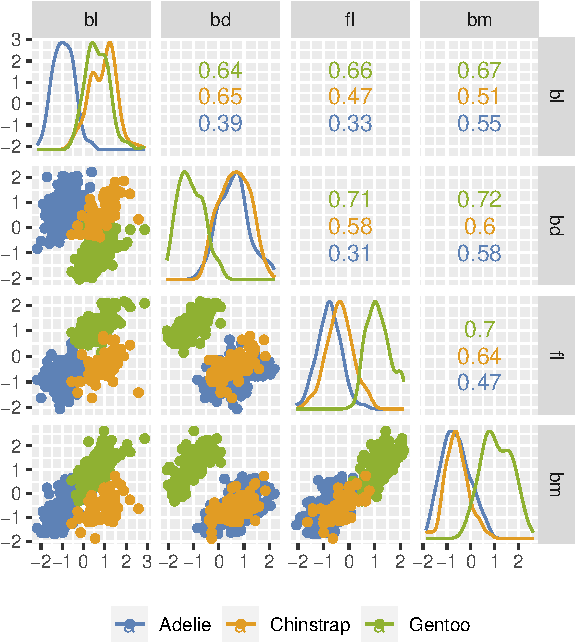
\includegraphics[width=0.6\linewidth]{paper_files/figure-latex/penguins-scatmat-1} 

}

\caption{Scatterplot matrix of the (standardized) penguins data. The three species are reasonably different in size, with Gentoo distinguished from the other two on bill depth relative to flipper length and body mass.}\label{fig:penguins-scatmat}
\end{figure}

To illustrate the usefulness of the manual controls we use the 4D
penguins data \citep{penguins} and look at classification models
following \citet{sam11271}. We will show how classification boundaries
can be explored and better understood on projections and slices through
4D space. Figure \ref{fig:penguins-scatmat} shows a scatterplot matrix
of this data. There are four variables
(\texttt{bl\ =\ bill\_length\_mm,\ bd\ =\ bill\_depth\_mm,\ fl\ =\ flipper\_length\_mm,\ bm\ =\ body\_mass\_g})
measuring the size of the penguins from three species (Adelie,
Chinstrap, and Gentoo). The scatterplot matrix shows that the three
species appear to be likely separable and that at least the Gentoo can
be distinguished from the other two species when \texttt{bd} is paired
with \texttt{fl} or \texttt{bm}. The steps for exploring boundaries in
this example are as follows:

\begin{enumerate}
\def\labelenumi{\arabic{enumi}.}
\tightlist
\item
  Build your classification model.
\item
  Predict the class for a dense grid of values covering the data space.
\item
  Examine projections, using a manual tour so that the contribution of
  any variable is controlled.
\item
  Slice through the center, to explore where the boundaries will likely
  meet.
\item
  Move the slice by changing the center in the direction of a single
  variable to explore the extent of a boundary for a single group
  relative to a variable.
\end{enumerate}

\hypertarget{constructing-the-4d-prediction-regions}{%
\subsection{Constructing the 4D prediction
regions}\label{constructing-the-4d-prediction-regions}}

We use the \texttt{classifly} package \citep{classifly} to generate
predictions across the 4D cube spanned by the data, with two
classification models: linear discriminant analysis (LDA) and random
forest (RF). Both the data and the model points in the grid are centered
and scaled (standard deviation \(= 1\)).

\hypertarget{exploring-projections-manually}{%
\subsection{Exploring projections
manually}\label{exploring-projections-manually}}

We start by exploring the projections of the model prediction. Figure
\ref{proj1} summarizes the process. Rotating manually the view, we can
visualize the location of predictions for each of the three species, and
also get a sense of the difference between the two models. To illustrate
this difference, we have manually rotated the projection for the RF
model (left plot) to identify a view that shows the non-linear but
block-type structure that is typical of this type of model. This
particular projection (\(A_1\)) is exported so that it can later be used
to show the LDA model (middle plot) and the actual data (right plot).
What can be seen is the linearity of the LDA model, where the boundaries
are linear and oblique to the variable axes. And, interestingly, this
particular projection of the original data shows very distinct clusters
of the three species. That means the obscuring of the boundaries between
groups for both of the models is driven by what is happening in the
orthogonal space to the plane of the selected projection.

\begin{figure*}[ht]
\centerline{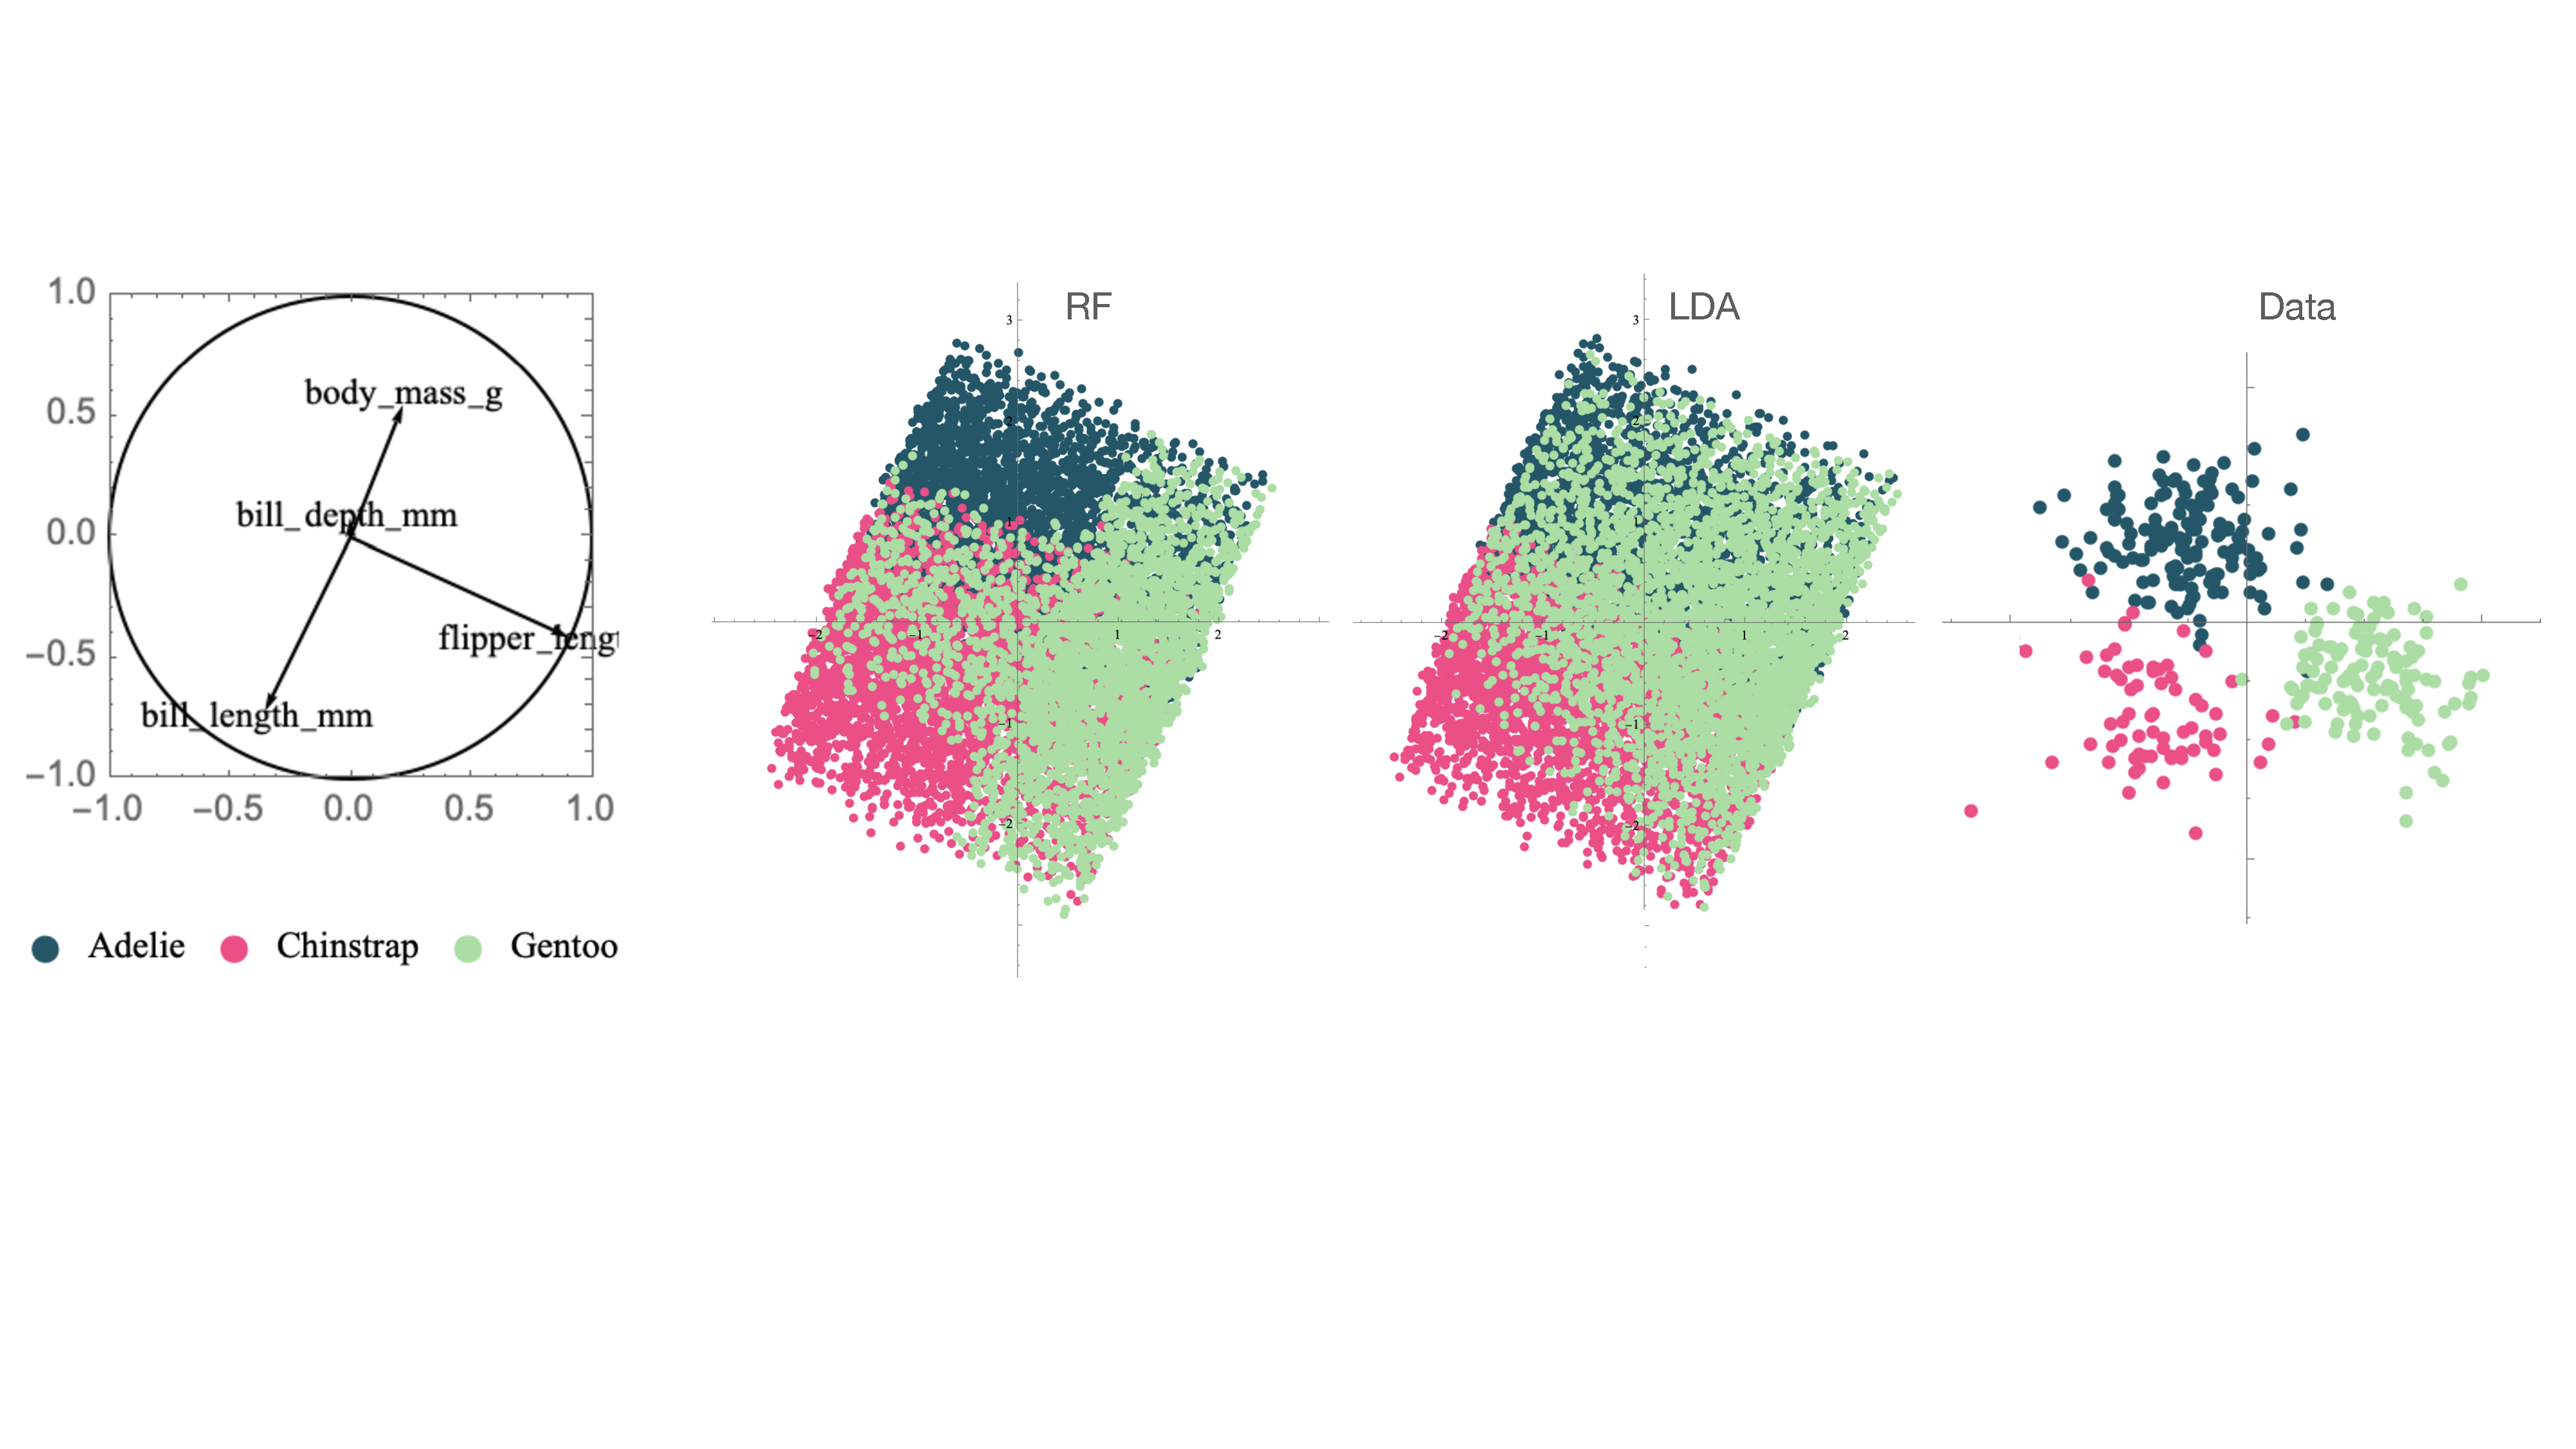
\includegraphics[width=0.95\textwidth]{figures/proj1.pdf}}
%\centerline{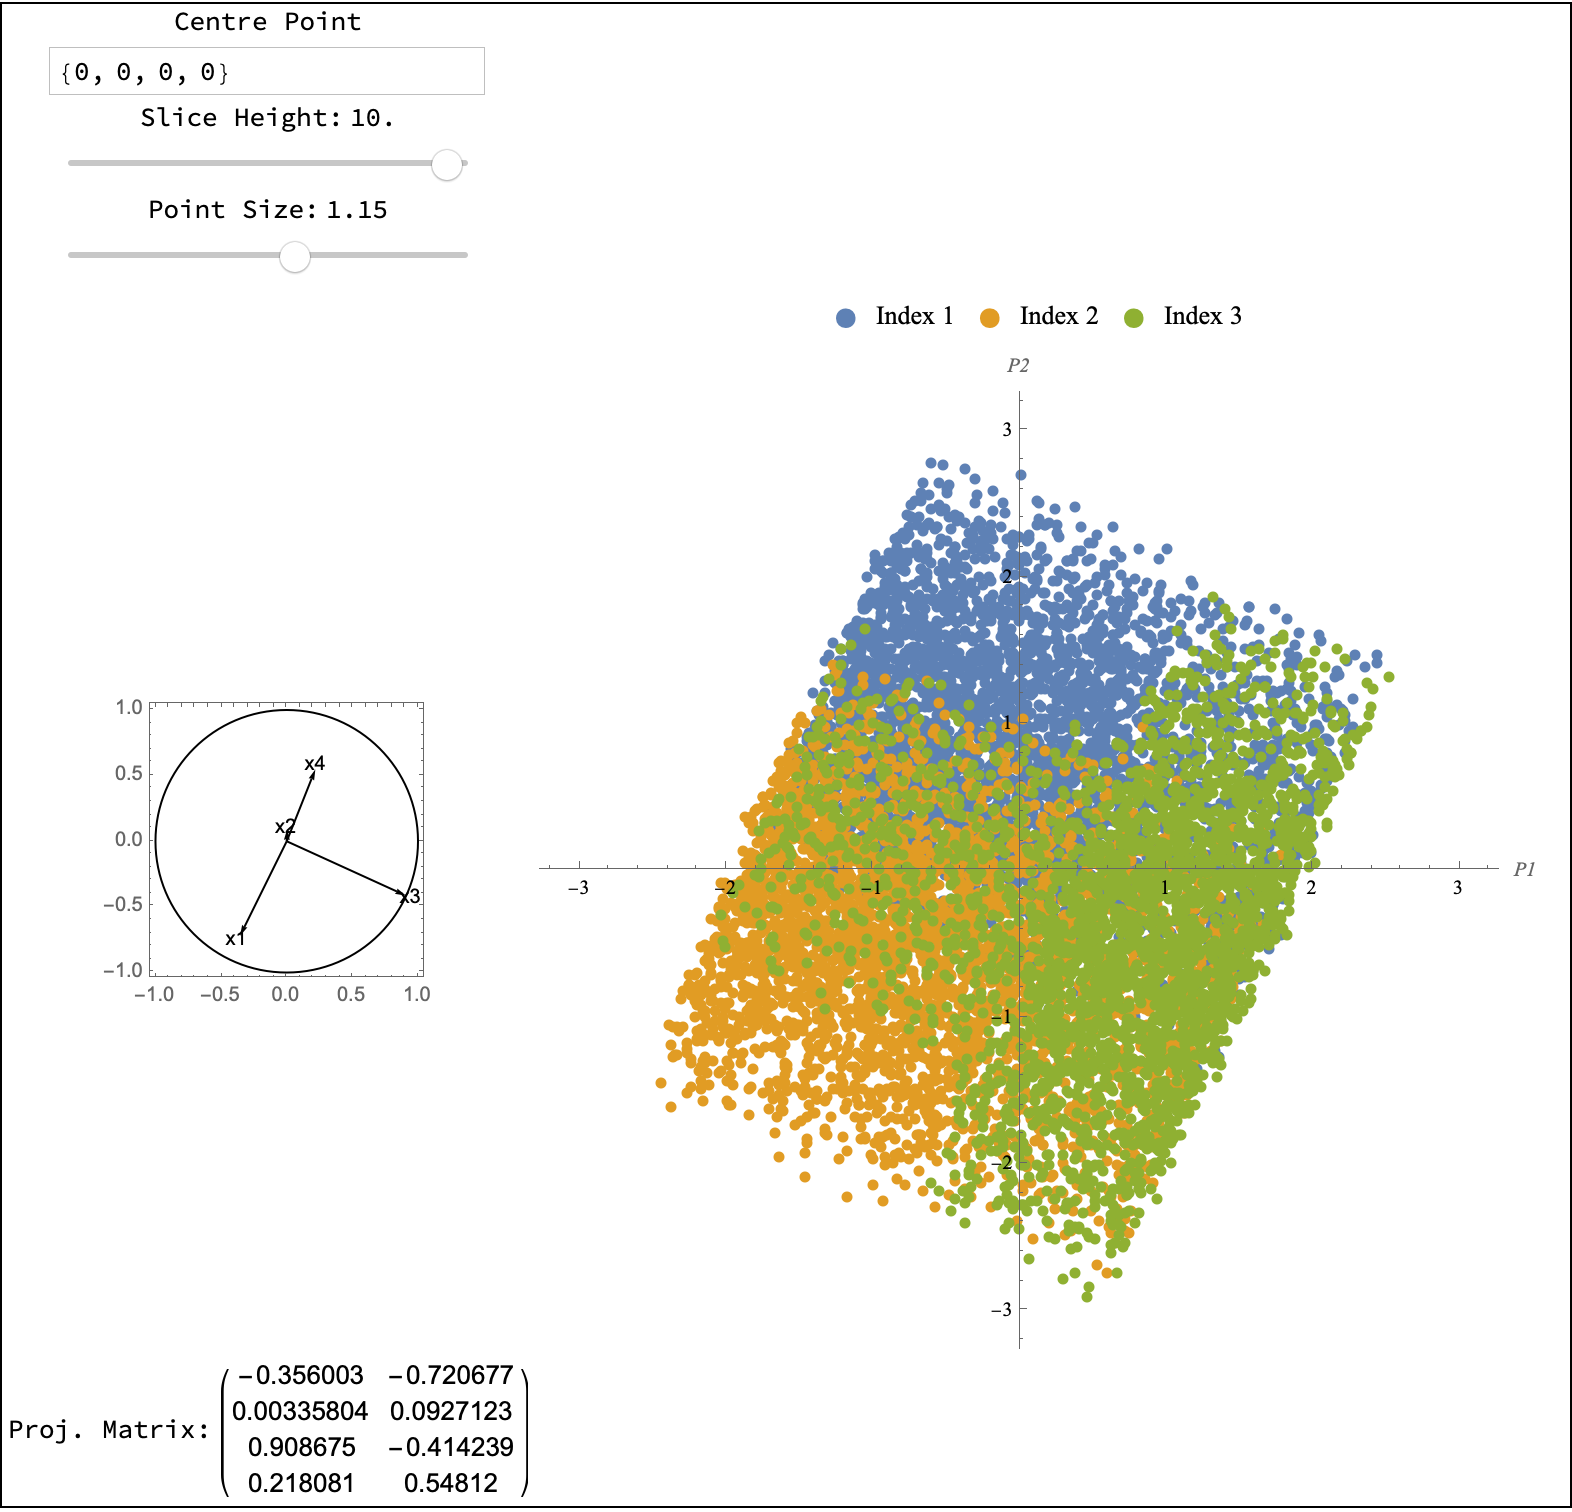
\includegraphics[width=0.32\textwidth]{figures/proj1_rf.png}
%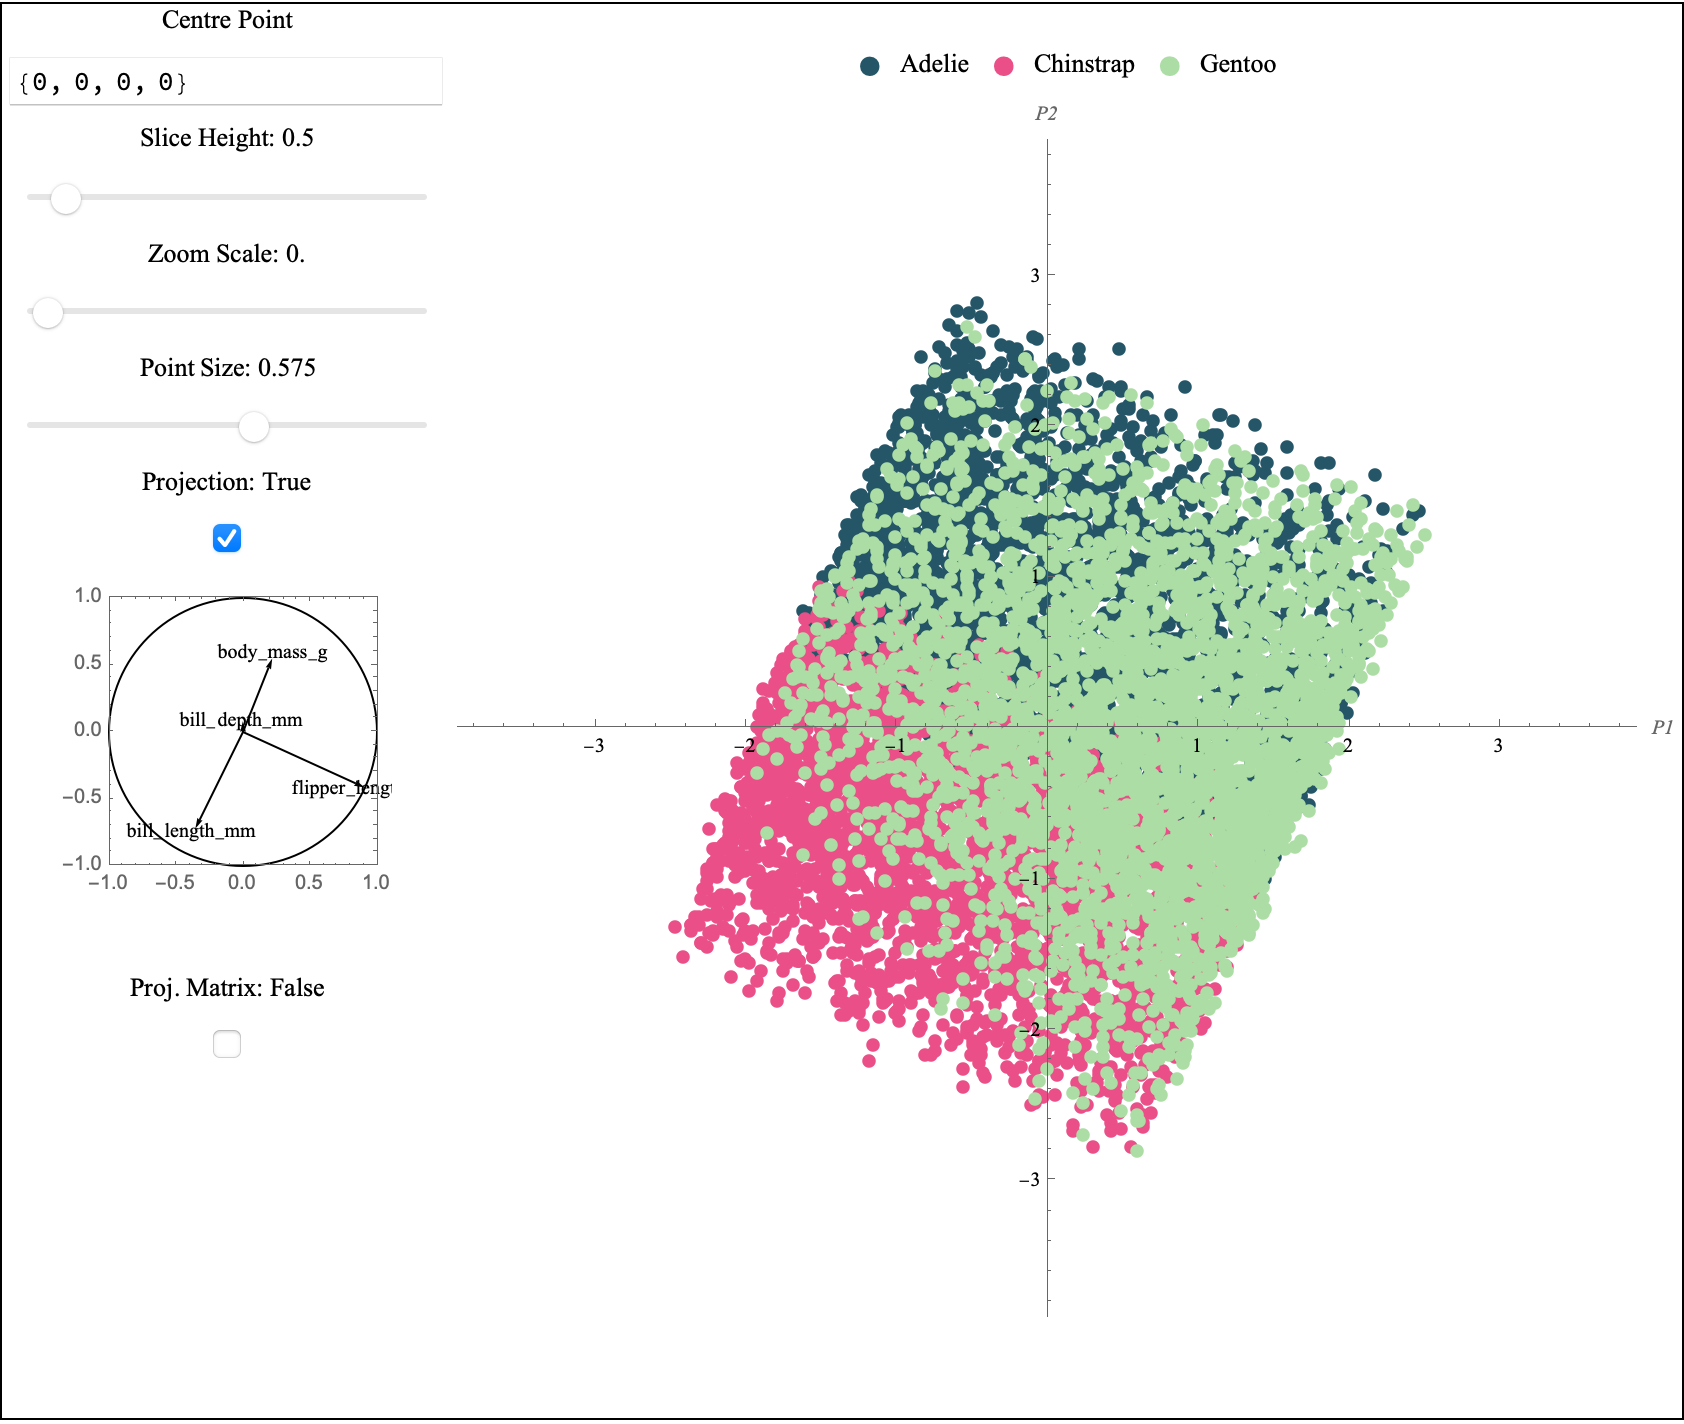
\includegraphics[width=0.32\textwidth]{figures/proj1_lda.png}
%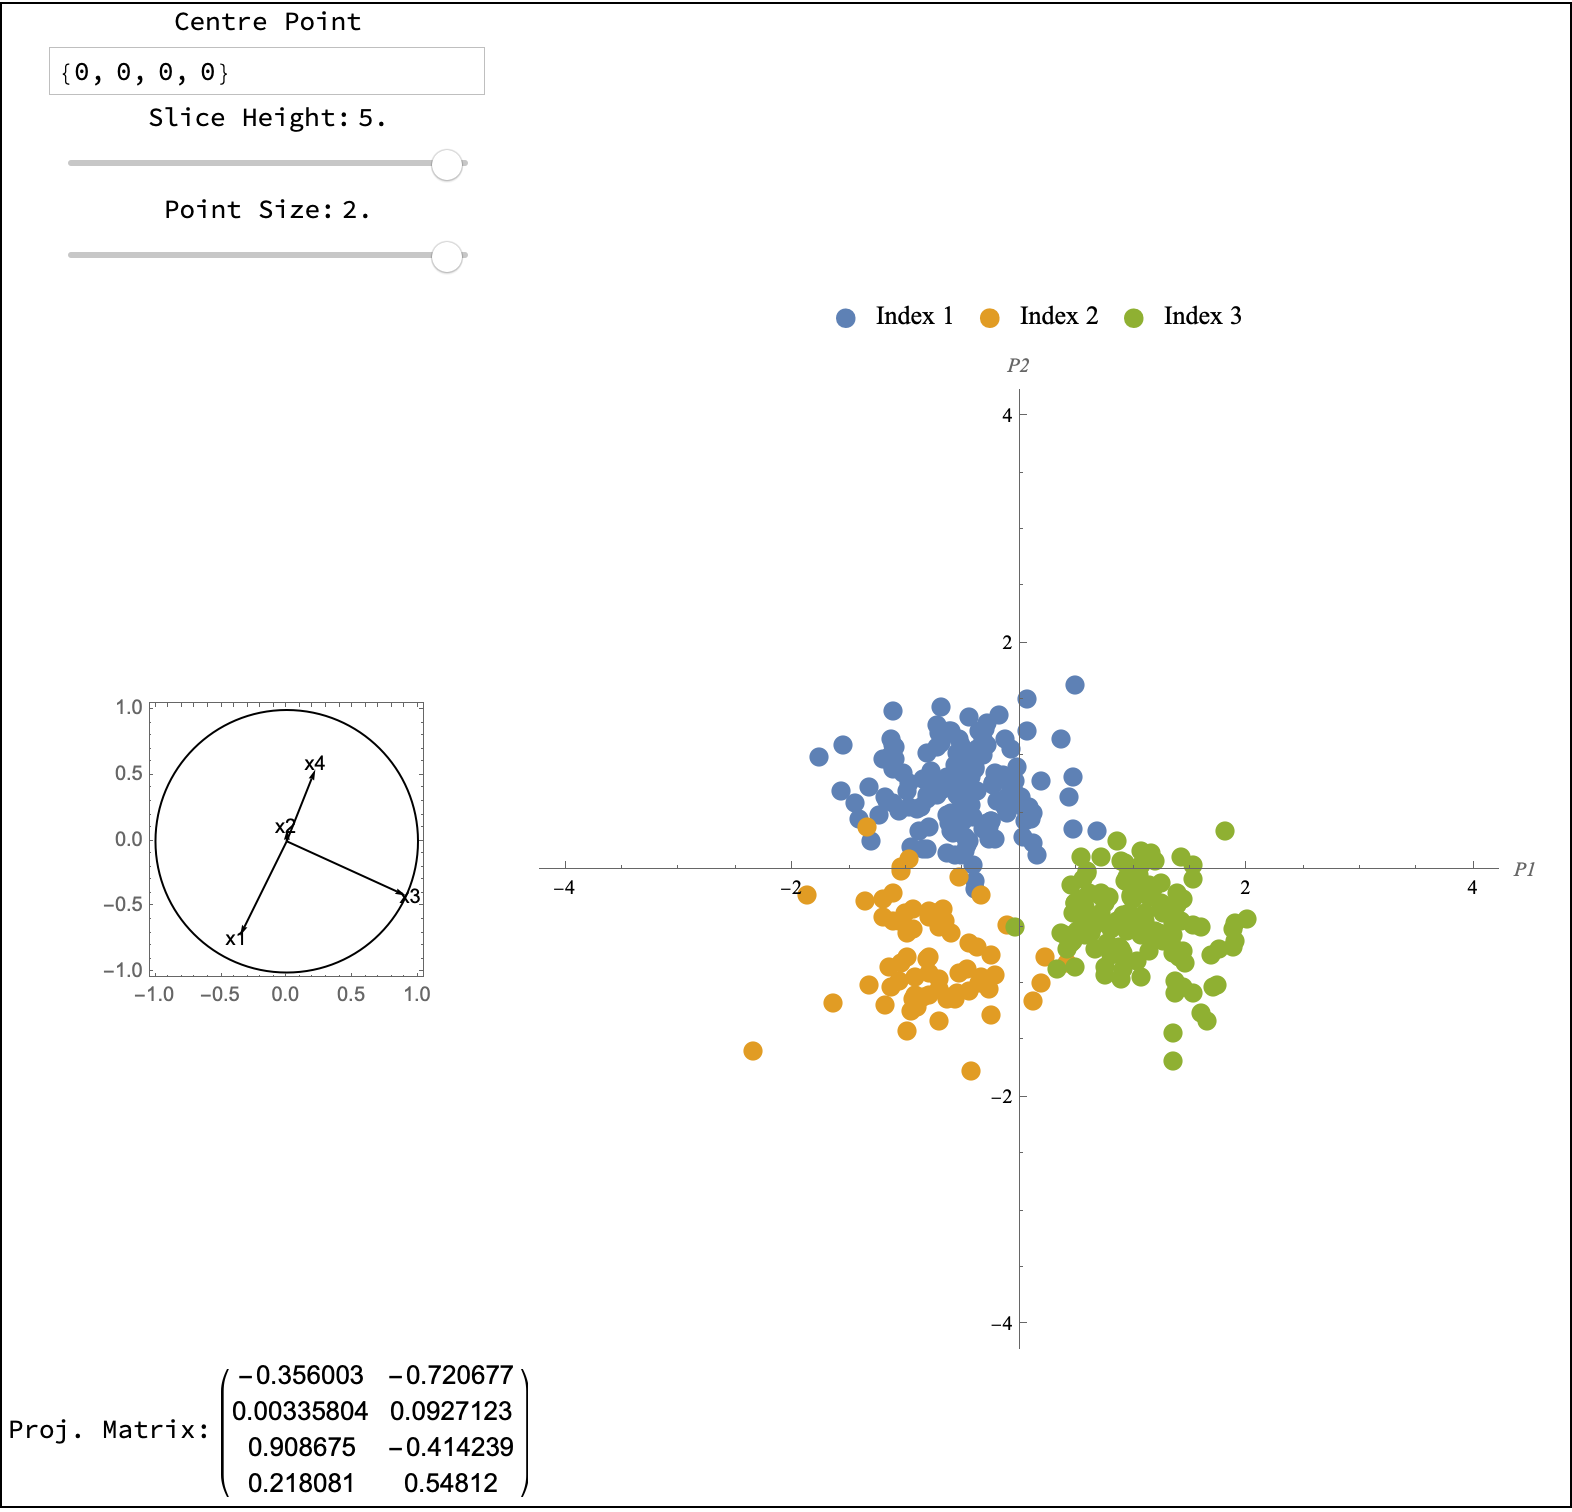
\includegraphics[width=0.32\textwidth]{figures/proj1_data.png}}
\caption{A projection identified using the manual tour because it shows differences in classification boundaries induced by different models. An RF model produces blocky, rectangular, boundaries, while the LDA model produces oblique linear boundaries. For comparison, in this projection, the data shows the three groups are almost perfectly separable.}
\label{proj1}
\end{figure*}

This example can be reproduced with the code in
penguins\_exploring\_manually.nb and a run-through is shown in the video
at \url{https://vimeo.com/747585410}.

\hypertarget{slicing-through-the-center}{%
\subsection{Slicing through the
center}\label{slicing-through-the-center}}

We now continue the investigation by slicing orthogonally to the
projection \(A_1\). For both models we look at a thin (\(h=0.5\)) slice
through the center, \(\mathbf{c}^0 = (0,0,0,0)\). At first, we explore
how changing the projection away from \(A_1\) can help with
understanding the boundary better. For our example, notice that \(A_1\)
does not contain any contribution from the second variable
(\texttt{bd}), so we will first rotate this variable into the view.

Figure \ref{slice1} shows snapshots of the exploration. The top row is
the initial projection (\(A_1\) and \(\mathbf{c}^0\)), and the bottom
row is a later projection containing more of \texttt{bd} (new projection
\(A_2\) while keeping the center fixed at \(\mathbf{c}^0\)). The columns
correspond to the two models, with RF on the left and LDA on the right.

Both models have some overlap at the center for the thin slice based on
\(A_1\) (despite the small value for \(h\)). The second slice (based on
\(A_2\)) mostly resolves this overlap and reveals the primary
differences between the models. The boundary between Adelie and
Chinstrap is very similar for both models. The boundary between
Chinstrap and Gentoo is where they differ.

The RF is almost straight in this view, as something we might expect
from a tree model where splitting occurs on single variables only.
However, it is straight in a combination of the second and third
variables (\texttt{bd} and \texttt{fl}). By examining the scatterplot
matrix, we can understand how this boundary was built: on each of
\texttt{bd} and \texttt{fl}, it is possible to cut on a value where most
of the Gentoo penguins are different from the other two species for any
tree, and likely only one is needed. Thus the forest construction is
providing a sample of trees that use one variable or the other variable
to split, producing the blocky boundary on the combination of the two.

In contrast, the LDA boundary has an oblique split between the two and
roughly divides the space into three similarly sized areas. It is almost
like a textbook illustration of how LDA works for two variables (2D)
where by assuming the clusters have equal variance-covariance, it places
a boundary halfway between the group means.

\begin{figure*}[ht]
\centerline{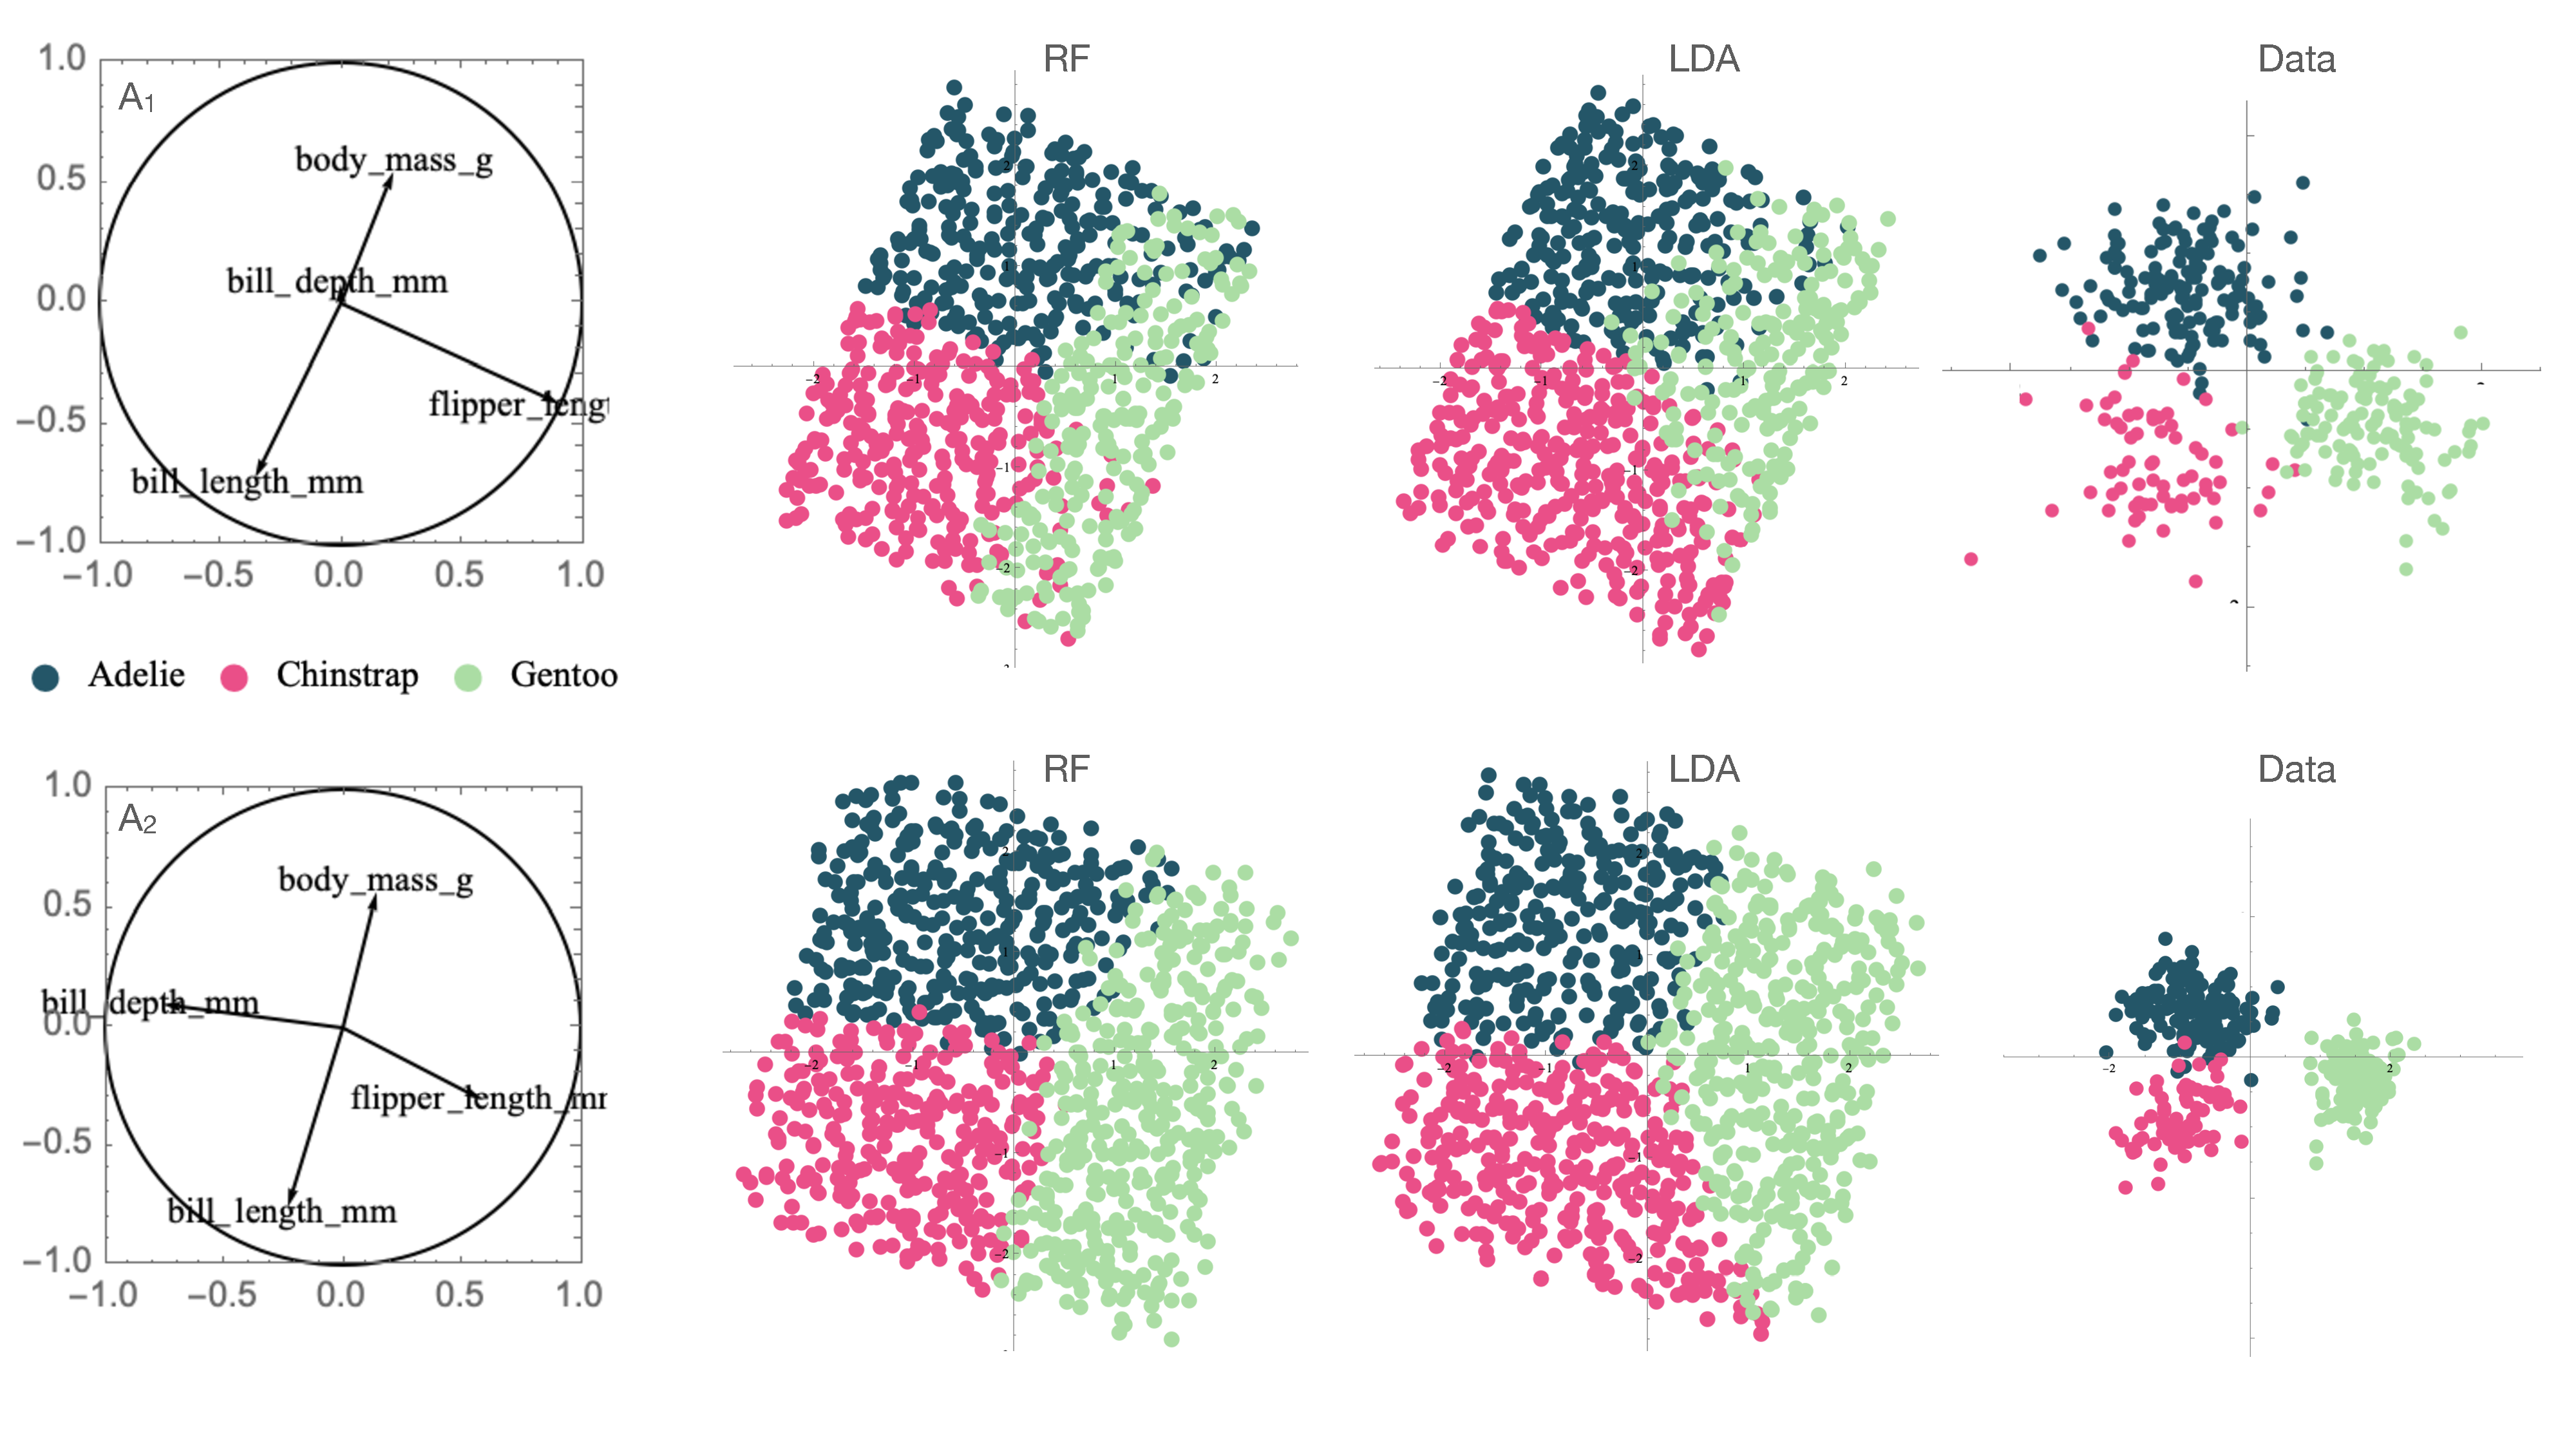
\includegraphics[width=0.95\textwidth]{figures/proj2.pdf}}
%\centerline{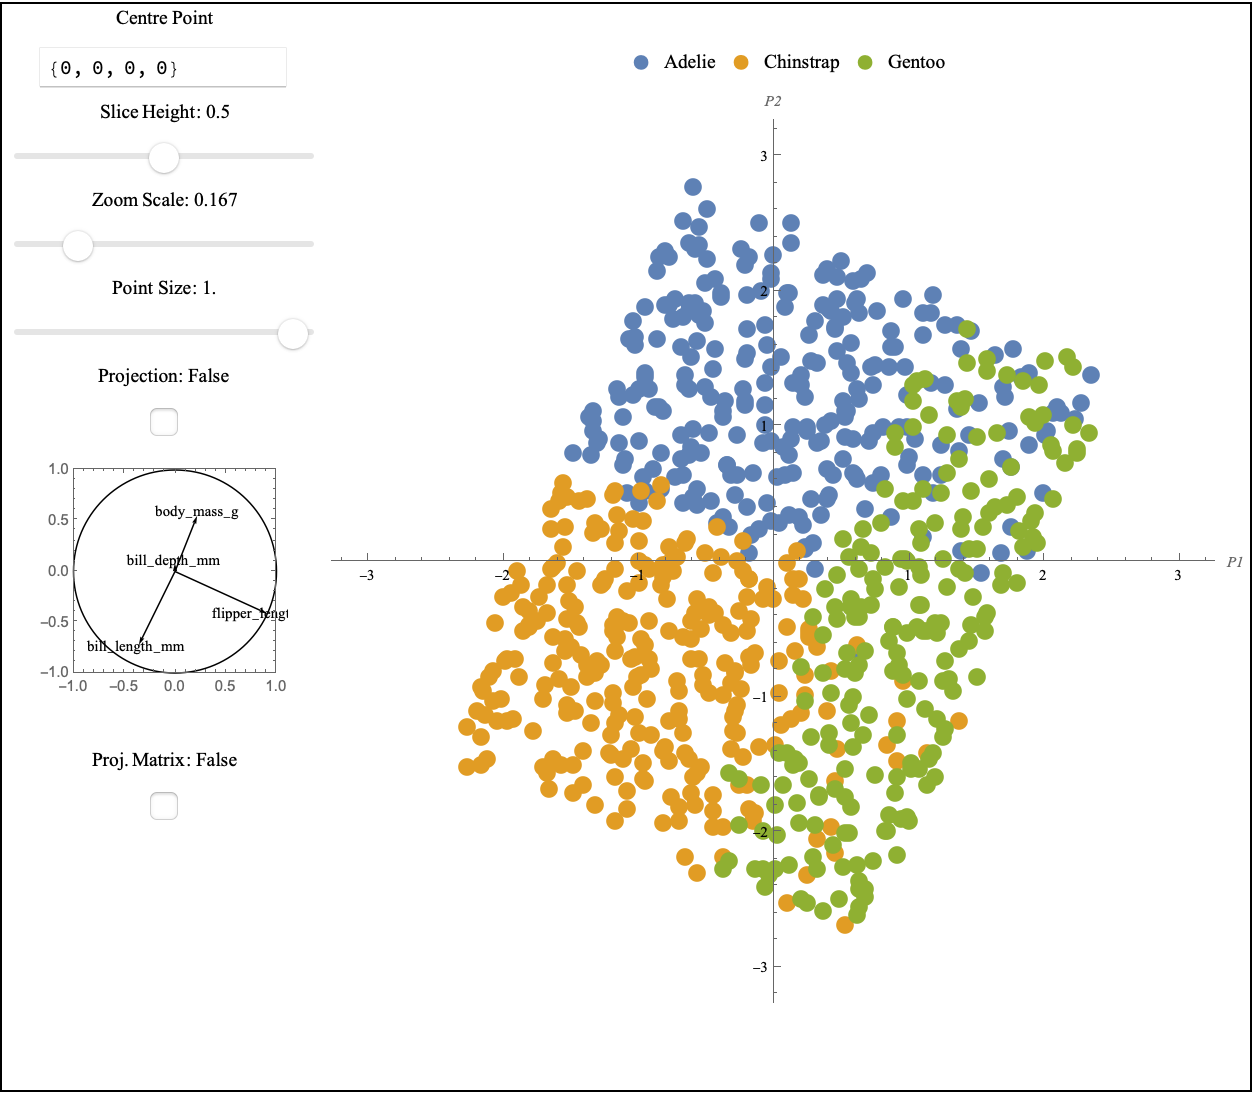
\includegraphics[width=0.45\textwidth]{figures/slice1_rf.png}
%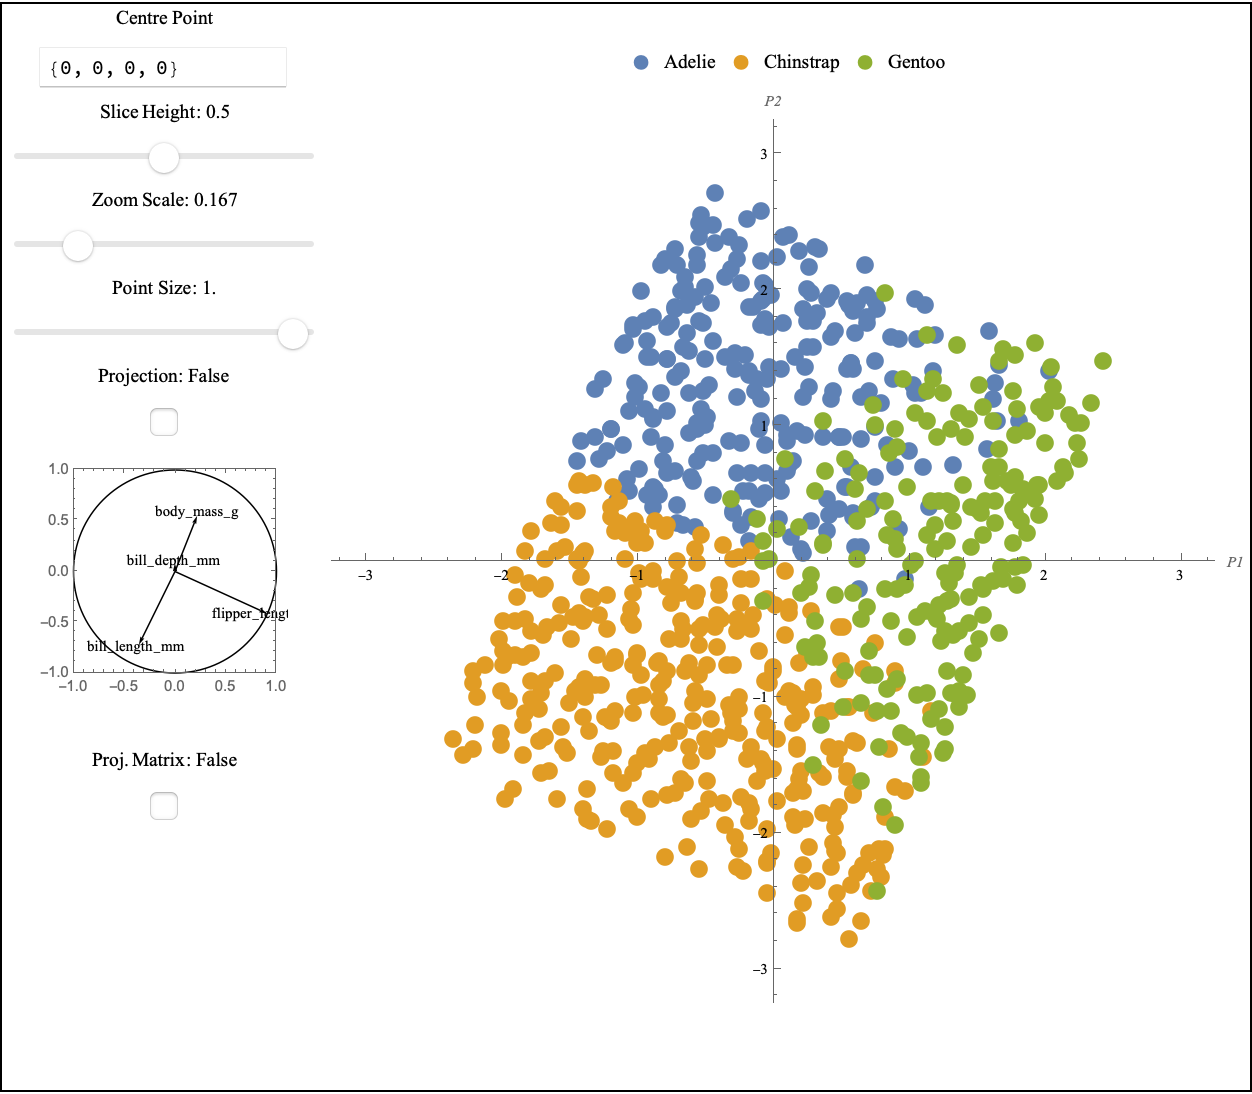
\includegraphics[width=0.45\textwidth]{figures/slice1_lda.png}}
%\centerline{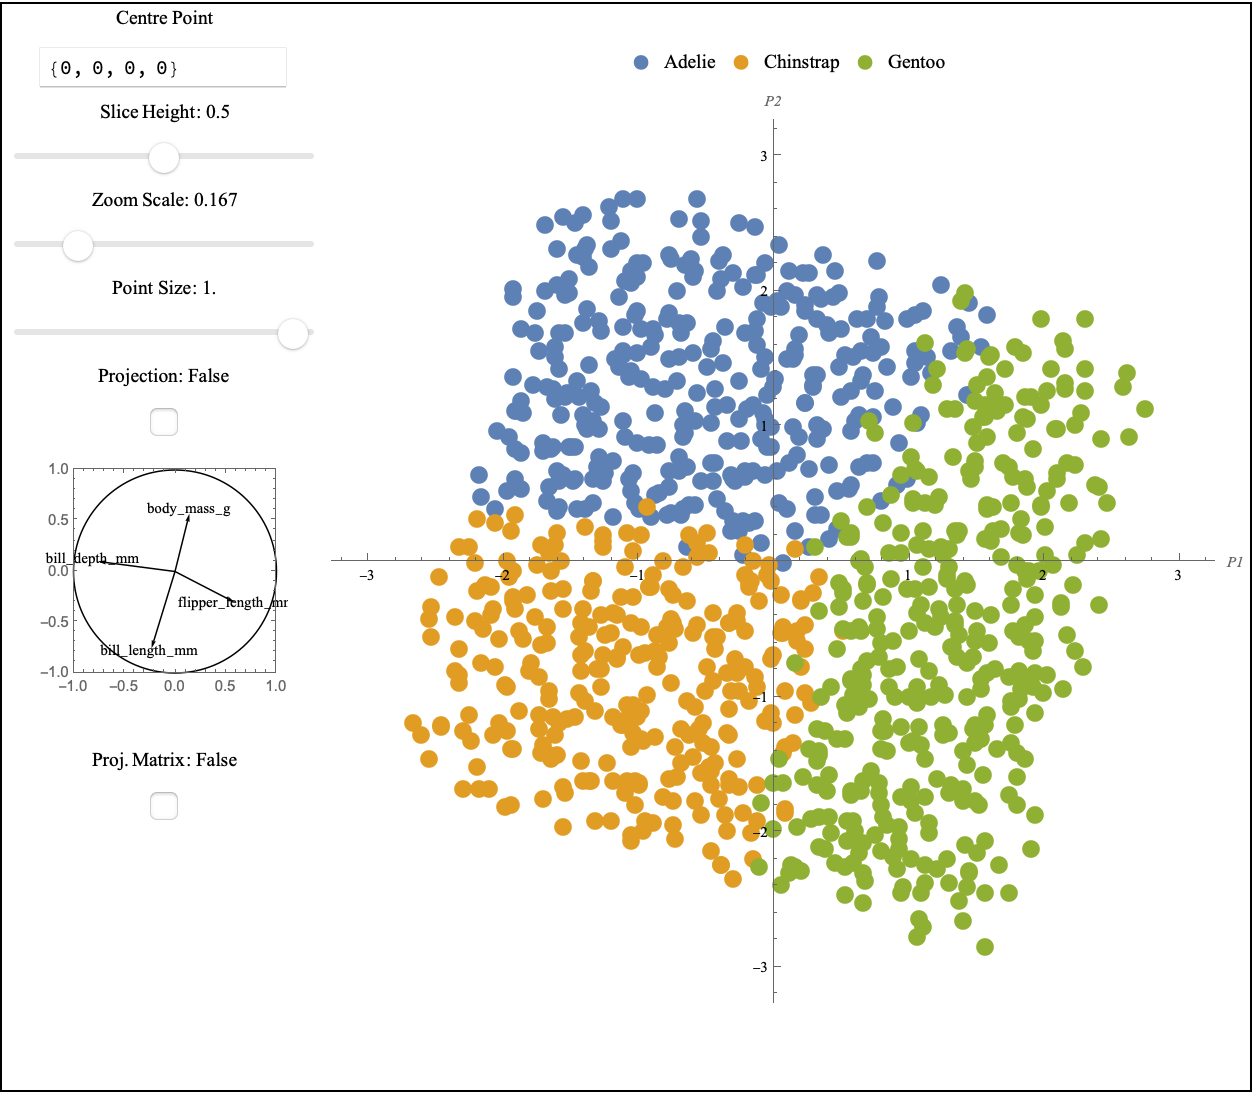
\includegraphics[width=0.45\textwidth]{figures/slice2_rf.png}
%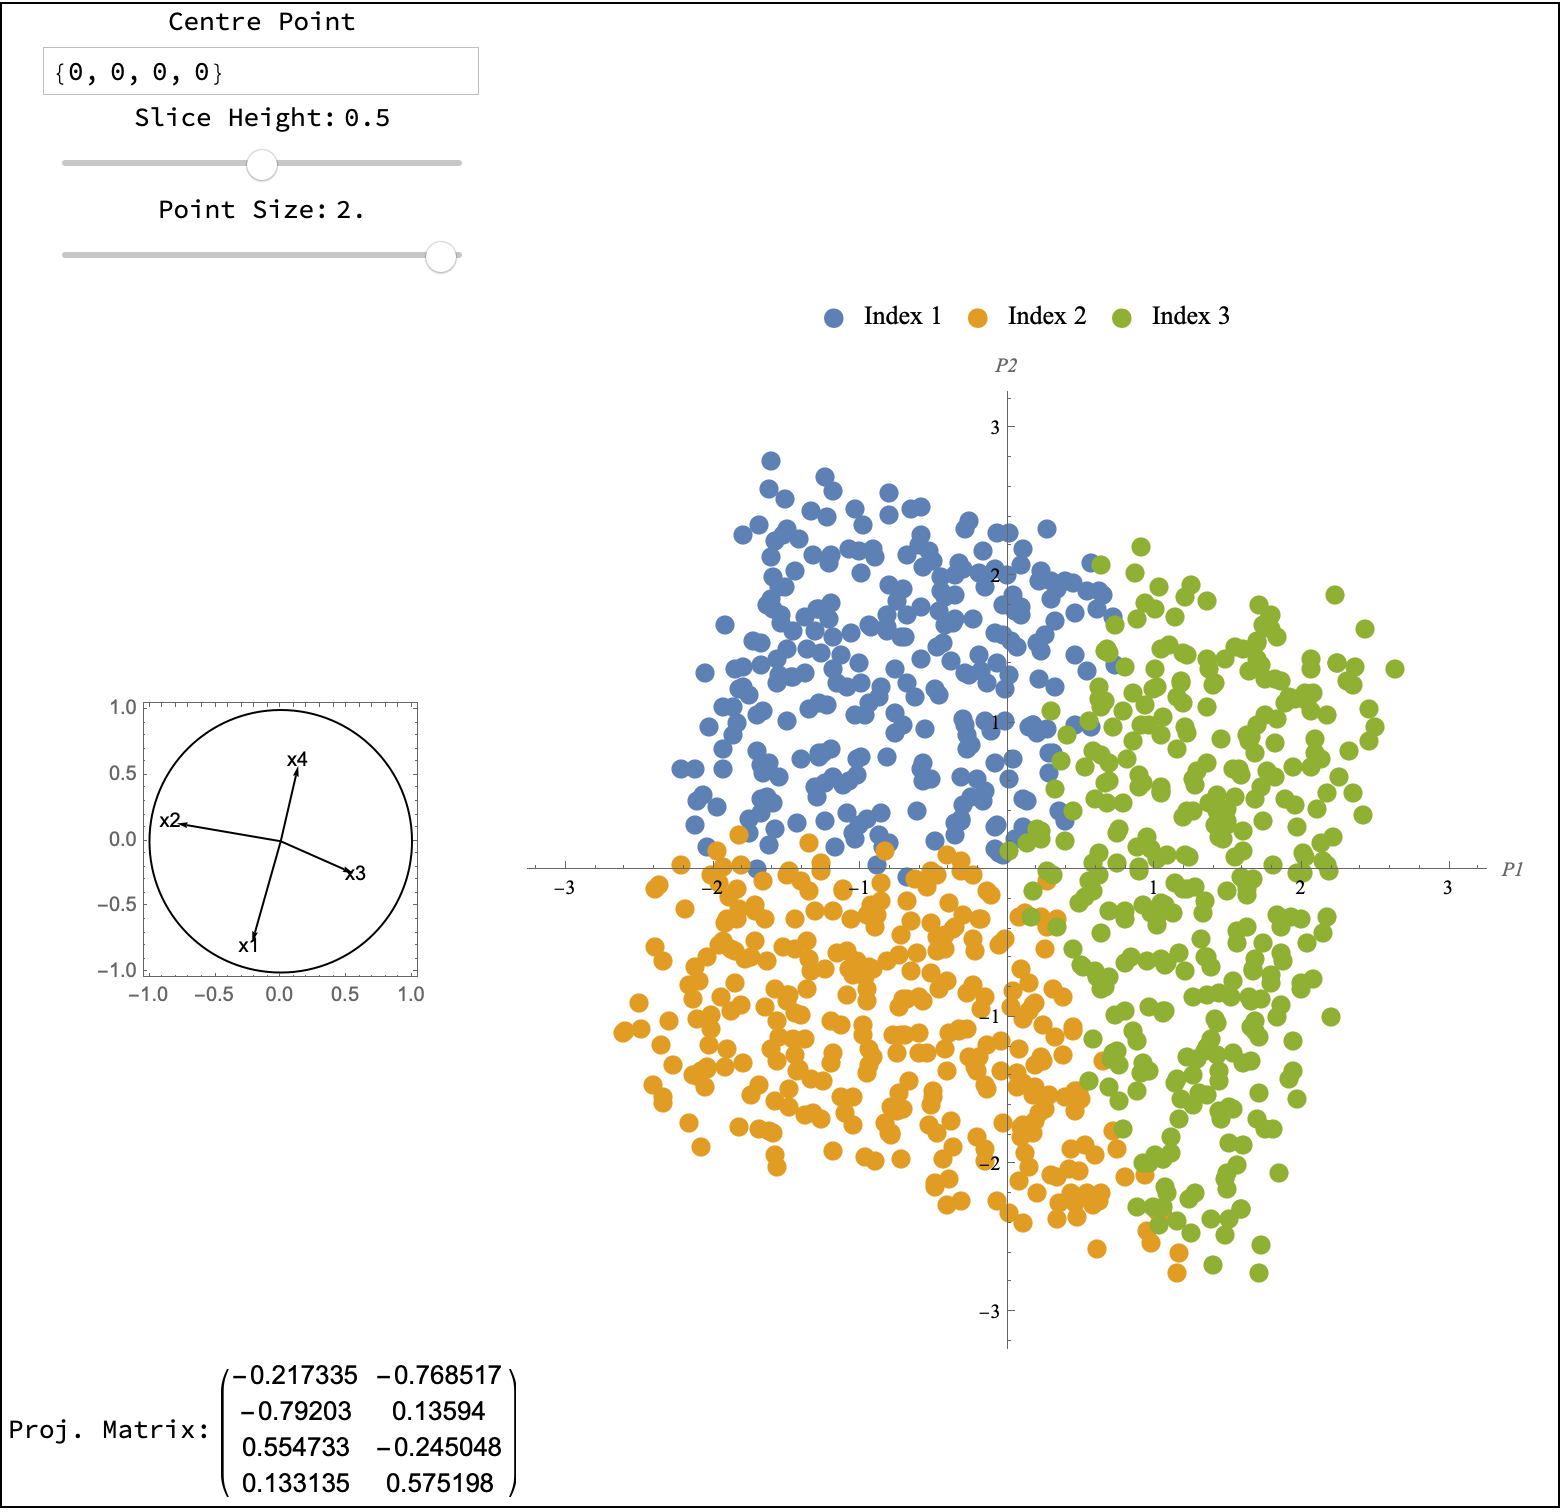
\includegraphics[width=0.45\textwidth]{figures/slice2_lda.png}}
\caption{Comparing slices from two different projections $A_1$ (top row) and $A_2$ (bottom row), to compare and contrast classification boundaries induced by two models RF and LDA. A thin slice through the center of the data is shown. The plot of the data shows that the Gentoo group (light grey/green) is less separated in $A_1$, and the rotation to $A_2$ produces a bigger gap. The boundaries between groups are clear in $A_2$ also. The LDA boundary is more oblique between Gentoo and Chinstrap than the RF, which is too close to the Chinstrap group. On the other hand between Adelie and Gentoo, the RF is better situated about halfway between the two groups. Interestingly, the RF boundaries, which can be highly nonlinear, albeit blocky, are relatively linear for this problem. }
\label{slice1}
\end{figure*}

Finally, to determine which model describes the boundaries better,
compare them with the \(A_2\) projection of the data (bottom row of
Figure \ref{slice1}). Gentoo is more separated from the other two in
this projection, and one can imagine that the trees in the forest have
greedily grasped any one of many places to make a split to separate the
group. It might be argued though the that RF boundary is cut too close
to the Chinstrap species, and might lead to some unnecessary
misclassification with new data. The LDA boundary is better placed for
all species.

This example can be reproduced with the code in
\texttt{penguins\_slicing\_through\_center.nb} and a run-through is
shown in the first part of the video at
\url{https://vimeo.com/747590472}.

\hypertarget{shifting-the-slice-center}{%
\subsection{Shifting the slice center}\label{shifting-the-slice-center}}

We have seen that starting from \(A_1\) using the manual controls to
change the contribution of the second variable we could find a clear
separation boundary indicating the relation between this variable (bill
depth) and the Gentoo penguin species. Instead of rotating to a
different projection, we might also change the view by moving the slice
along one axis in the 4D space. Here we will continue our exploration of
the dependence on \texttt{bd} and move the slice defined by \(A_1\) to
either large positive or negative values (\(c^{\pm}_{bd} = \pm 1.5\)
after centering and scaling). Thus we define
\(\mathbf{c}^{\pm} = (0, c^{\pm}_{bd}, 0, 0)\). Here we will also look
at slices of the observed data points, using a thicker slice (\(h=1.5\))
to capture enough points in a given view.

We start with a comparison of the two models and the data distribution
shifting to \(\mathbf{c}^{+}\), thus the slice is localized towards high
values of bill depth in the top row of Figure \ref{slice1p}.
\textcolor{blue}{The star glyph at the right indicates the slice center value, which shows that it is higher on `bd` and at the middle value for the other variables. This slice center guide is as proposed in @condviz2, and more details can be found in the Appendix.}
We can see that all three slices (the two models and the data) contain
almost no points from the third class (Gentoo) and that the decision
boundary between the two models is very similar.

\begin{figure*}[ht]
\centerline{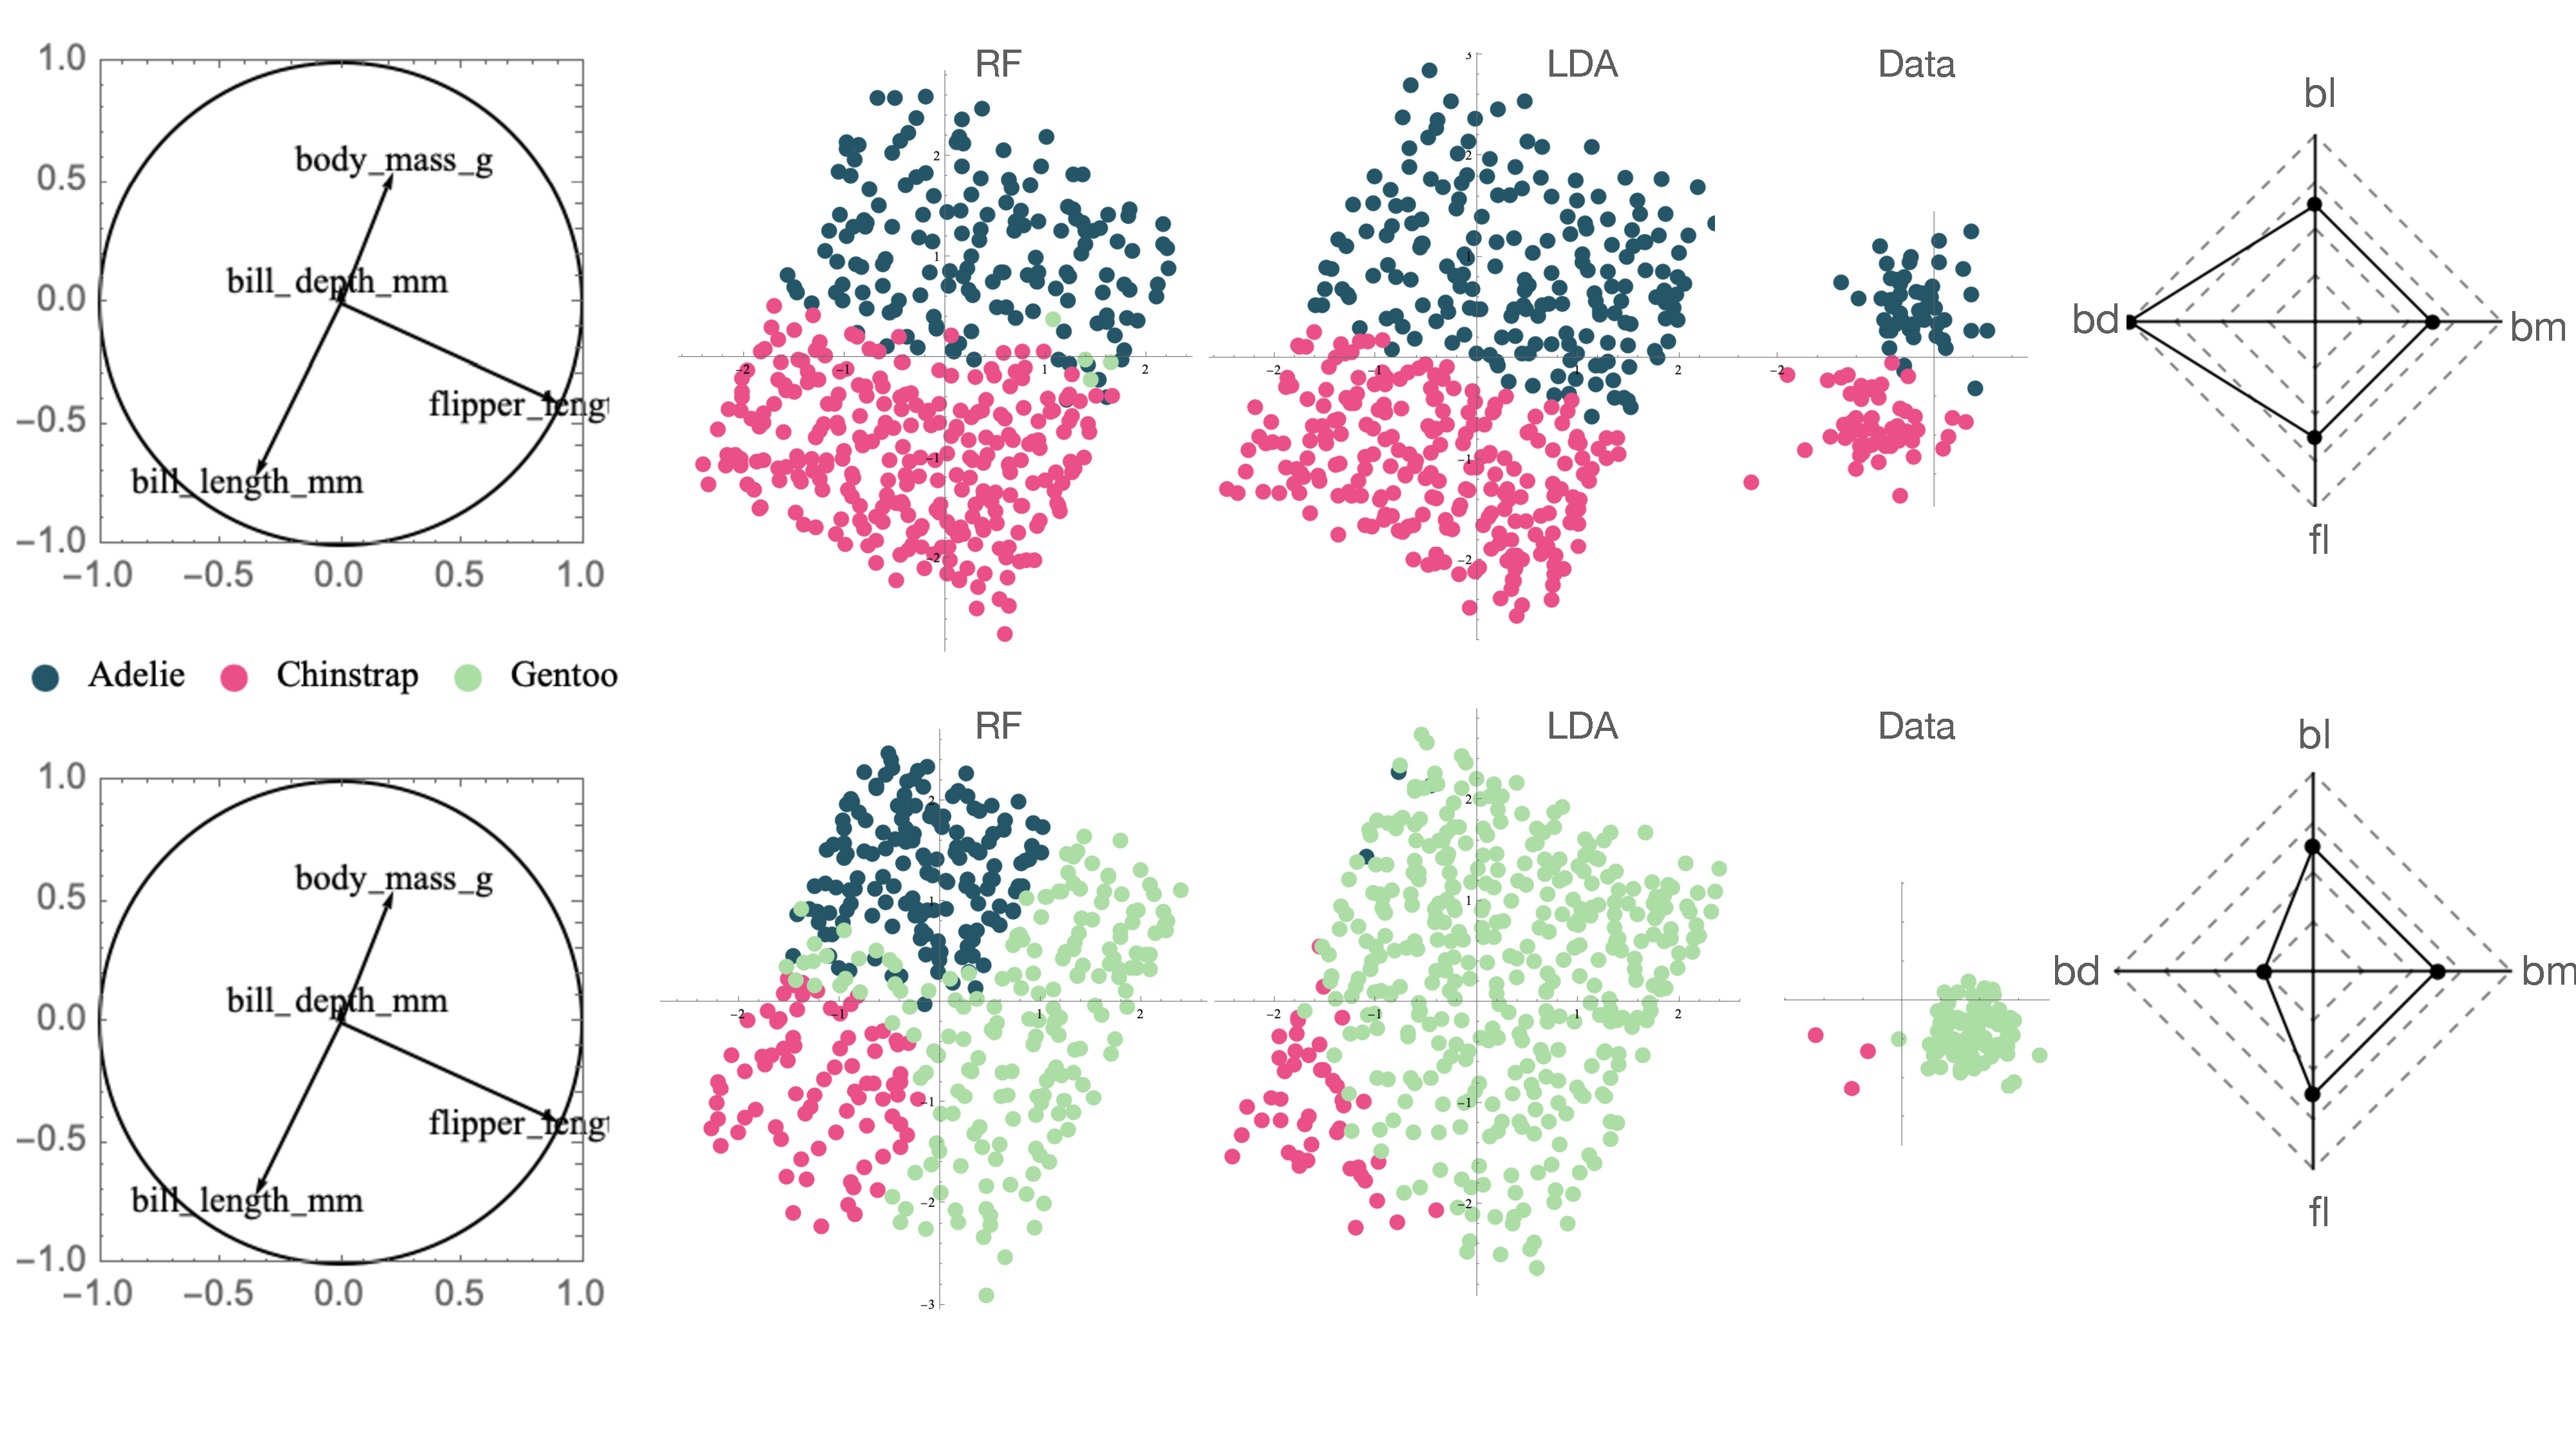
\includegraphics[width=0.95\textwidth]{figures/slice1_p.pdf}}
%\centerline{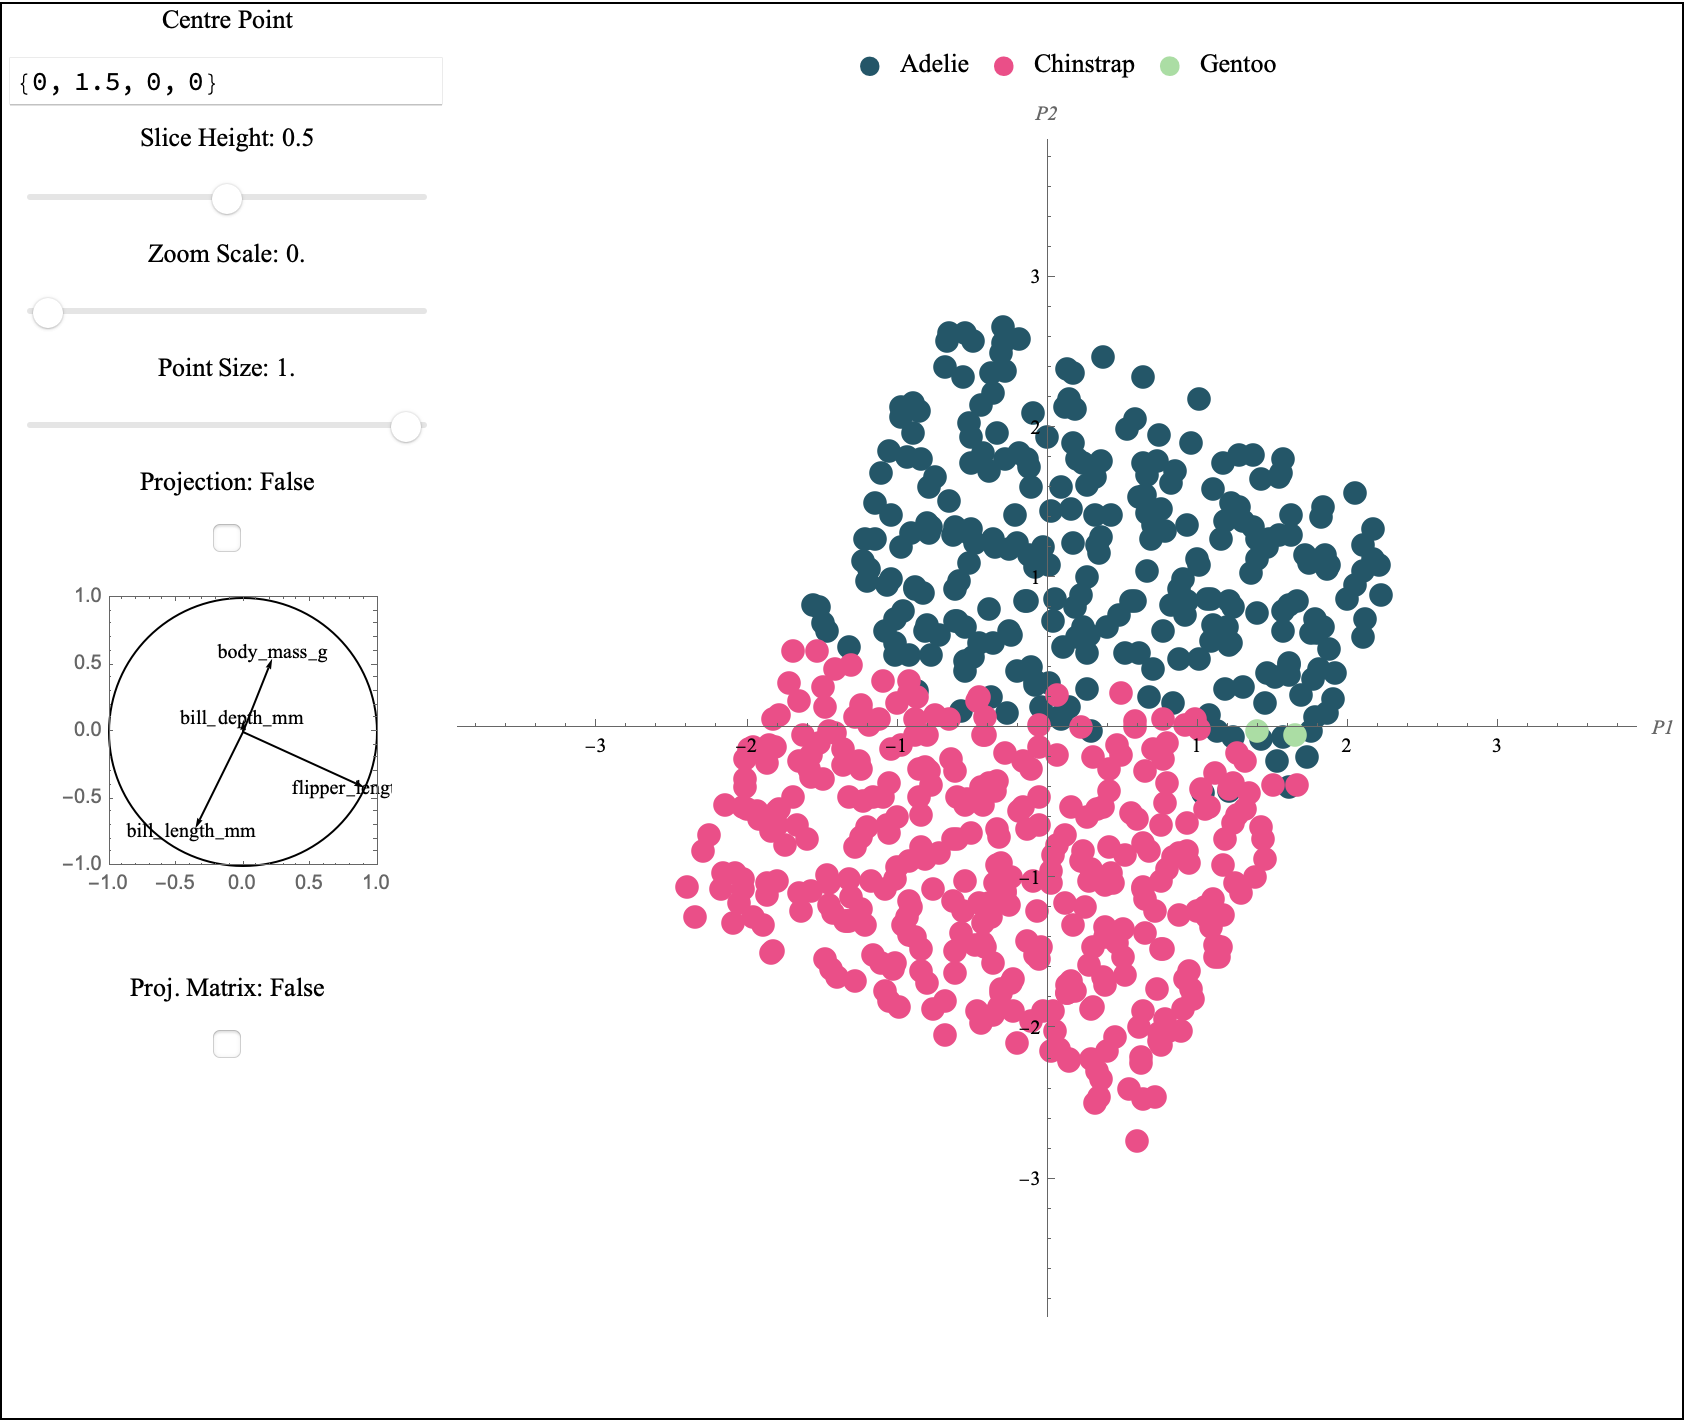
\includegraphics[width=0.32\textwidth]{figures/slice1_p_rf.png}
%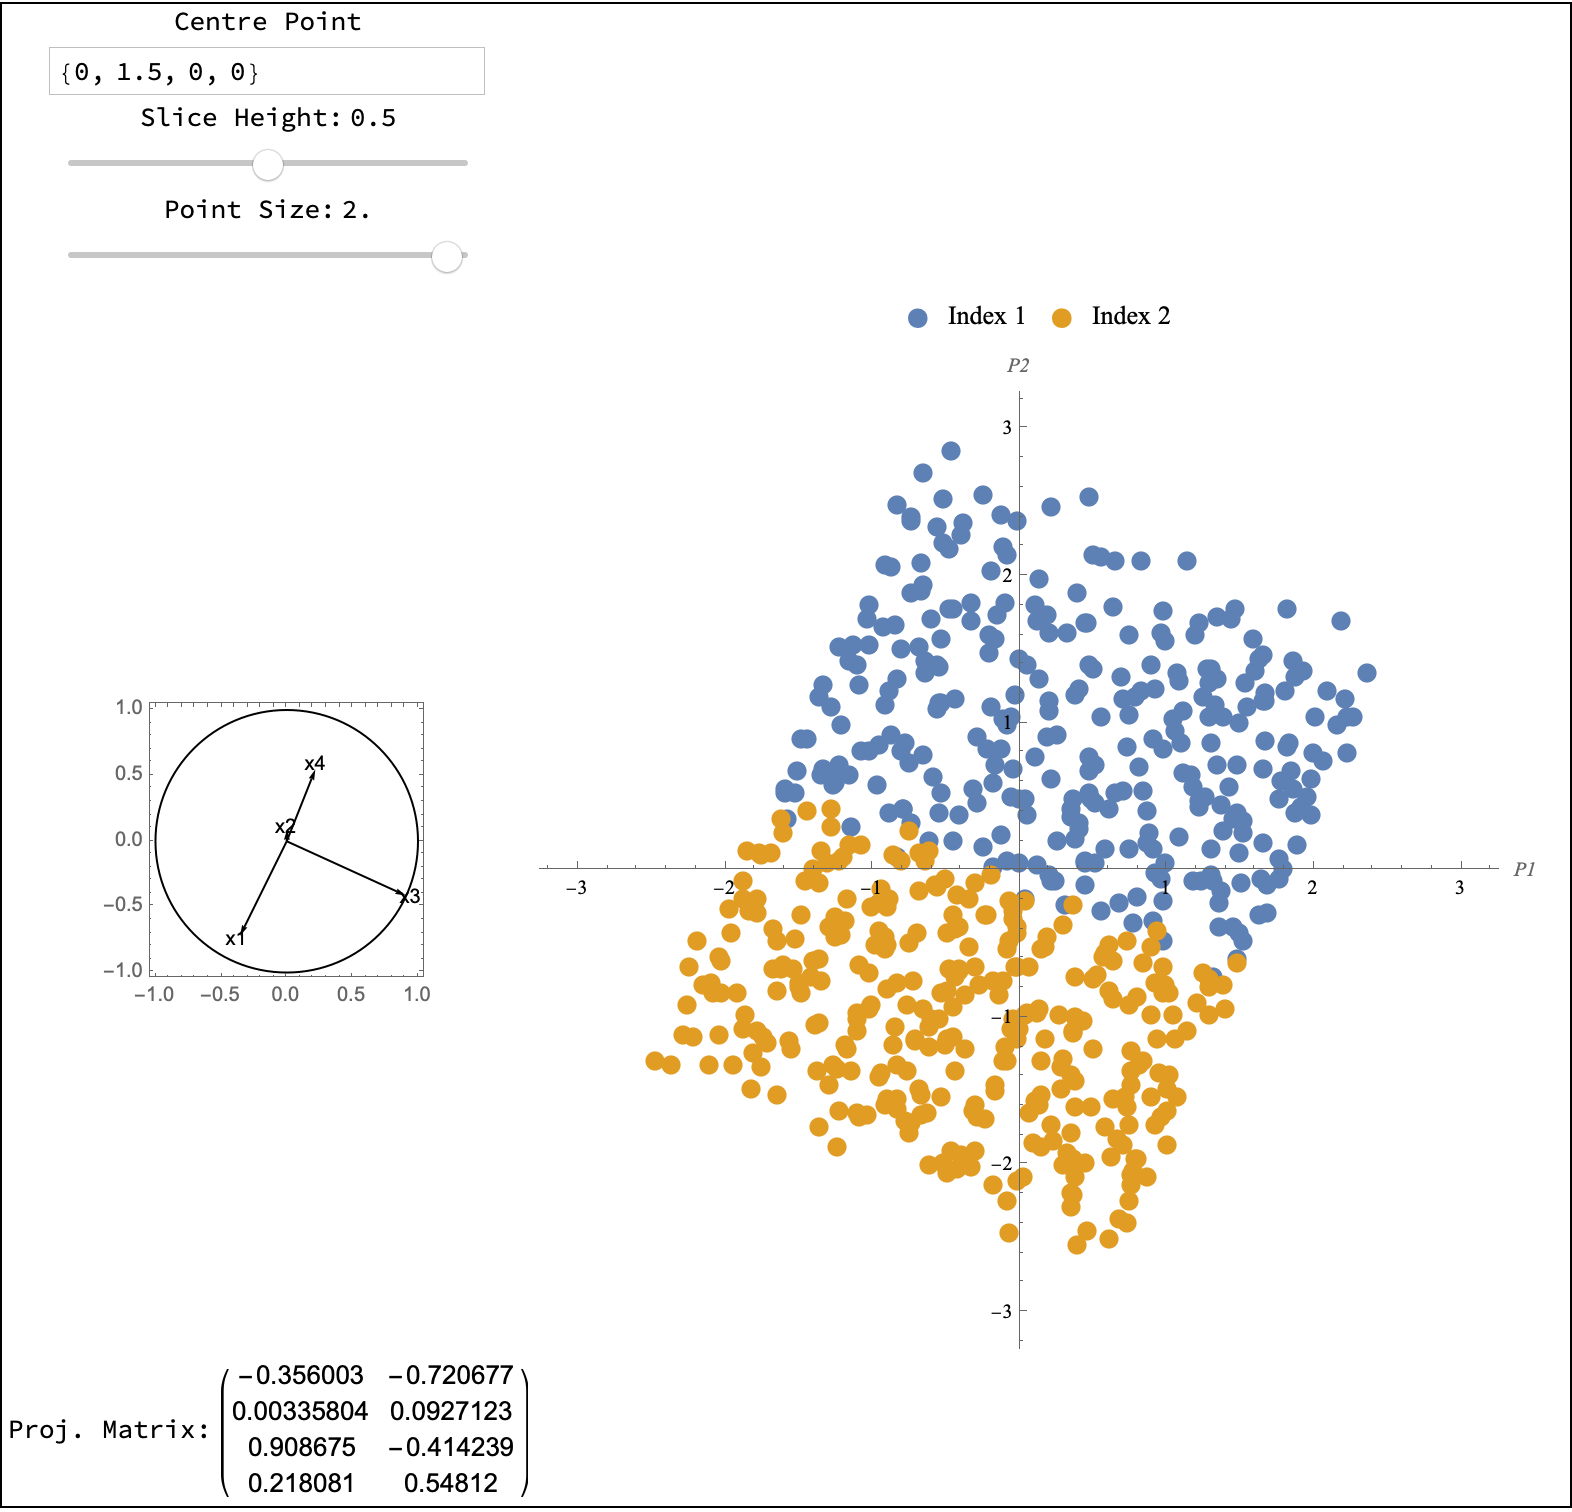
\includegraphics[width=0.32\textwidth]{figures/slice1_p_lda.png}
%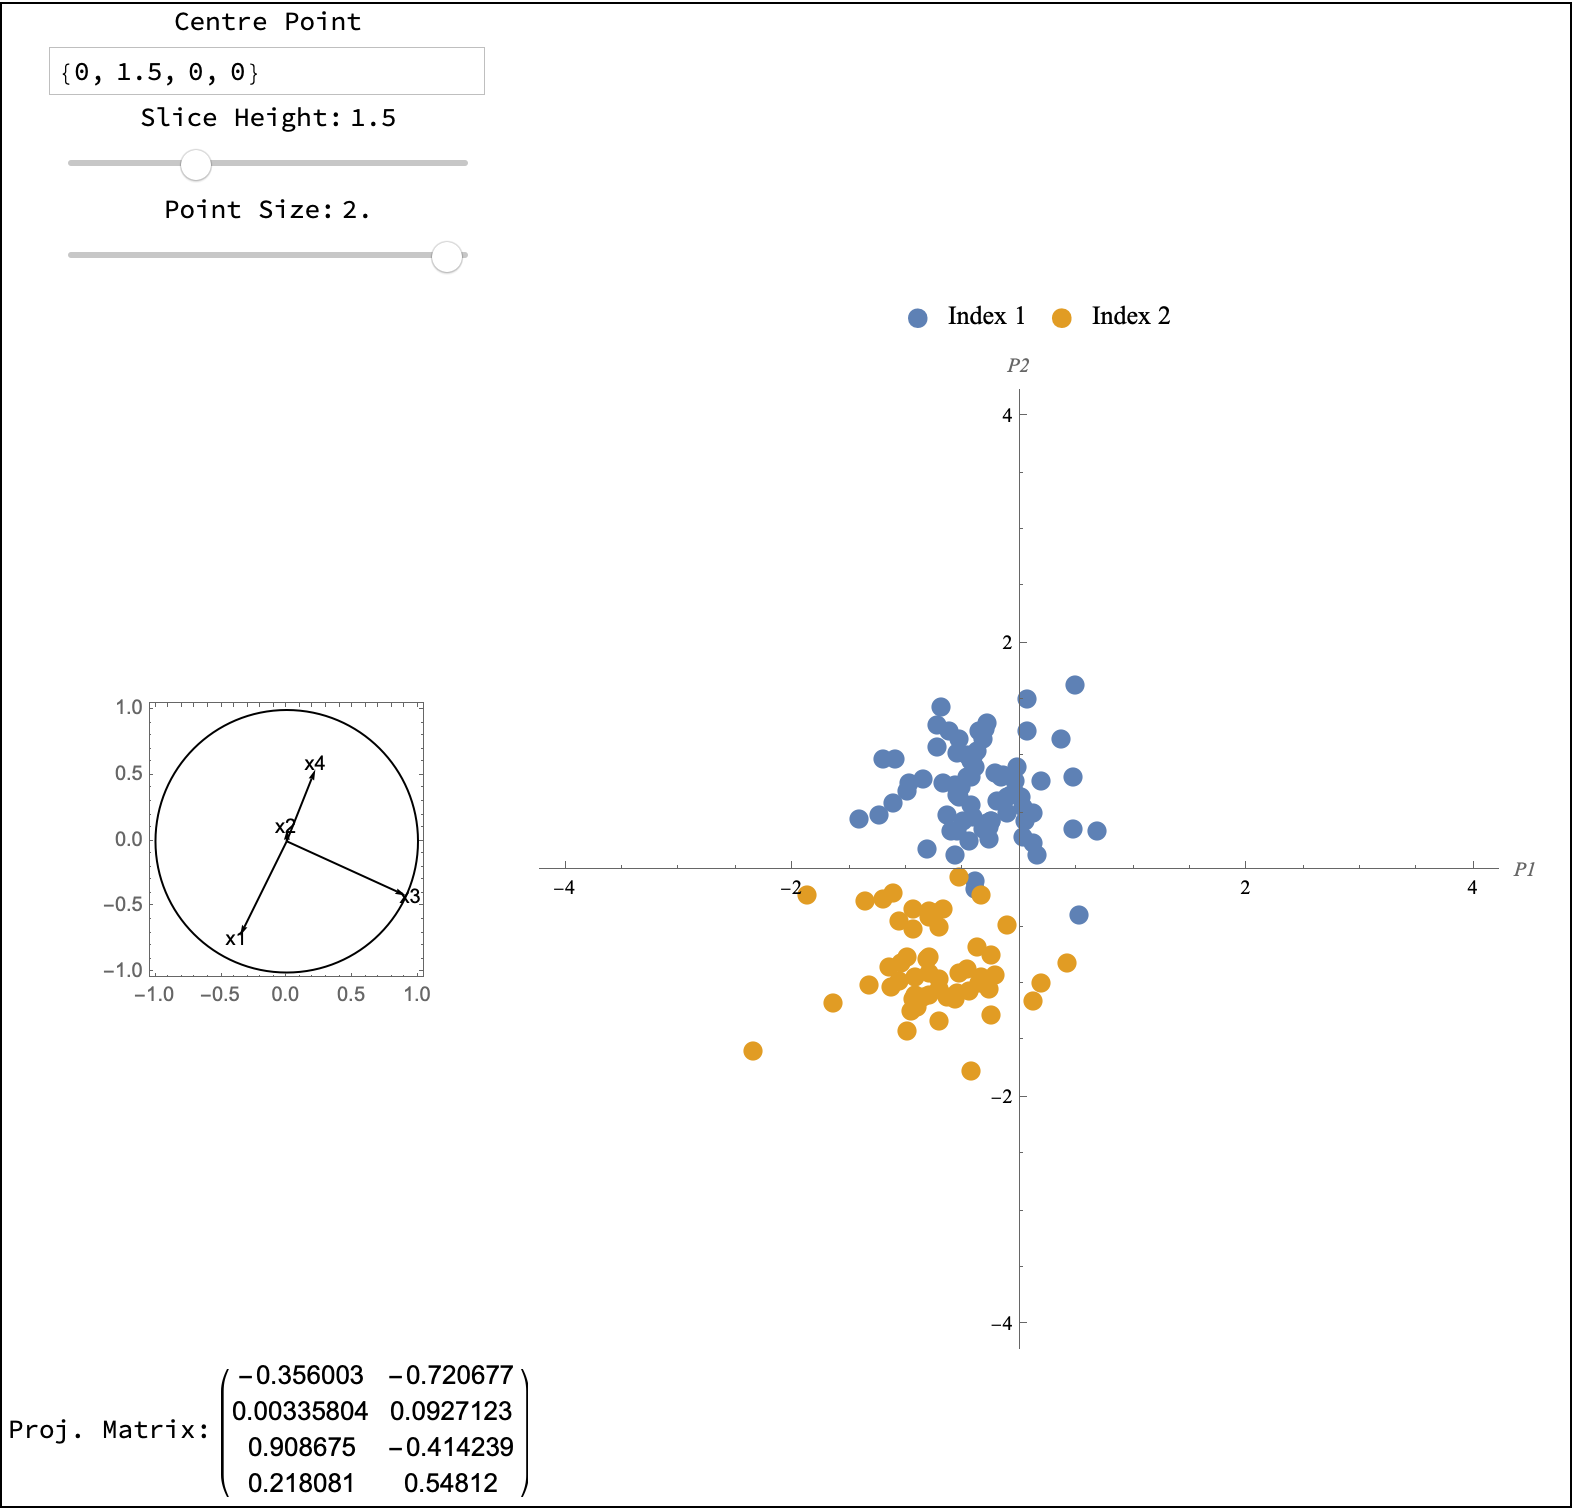
\includegraphics[width=0.32\textwidth]{figures/slice1_p_data.png}}
\caption{Shifting the slice center allows for exploring the boundary in different subspaces. Here the center has been shifted along the axis of `bd` (icon display at right represents slice center position). (Top row) The center is at large values of `bd`, showing a region with no Gentoo. The two models have similar boundaries except that the LDA is more linear. (Bottom row) The center is at small values of `bd`, revealing a region where the models differ substantially. The RF model carves some area for Adelie, but LDA would only predict to be Gentoo or Chinstrap here. LDA better matches the observed data in this region.}
\label{slice1p}
\end{figure*}

A more interesting comparison is found for \(\mathbf{c}^{-}\), thus the
slice localized towards low values of bill depth, shown in the bottom
row of Figure \ref{slice1p}.
\textcolor{blue}{(The star glyph at right indicates the slice center value, which shows that it is lower on `bd` and at the middle value for the other variables.)}
The RF model (left) predicts all three species within this slice, with
an interesting boundary for the third class (Gentoo). On the other hand,
the LDA model (middle) predominantly predicts the third class within the
slice, this appears to be enforced through the linear structure of the
model. Looking finally at the thick slice through the data we see that
there are primarily observations from this class within the slice we can
conclude that the two models have filled in the ``empty'' space (where
we do not have any training observations) in very different ways and
according to what we might expect given the model structure.

Finally, it is interesting to compare the slice views to the projection
of the models seen in Fig. \ref{proj1} to better understand how the
boundaries change along the \texttt{bd} direction and where the
differences in the projections come from.

This example can be reproduced with the code in
penguins\_shifting\_slice\_center.nb and a run-through is shown in the
second part of the video at \url{https://vimeo.com/747590472}.

\hypertarget{sec:discussion}{%
\section{Discussion}\label{sec:discussion}}

This short note has described new technology for manually interacting
with tours. The manual control of projection coefficients is most useful
for assessing variable importance to the perceived structure but can be
generally used for steering a viewer through high-dimensional space.
Changing the center of a slice manually enables exploring the space
orthogonal to a projection, specifically in the direction of a single
variable. This is a new tool, and as shown in the example, when used
with the slice tour can be very useful for understanding the boundaries
of classifiers. This is also likely a useful method for examining
low-dimensional non-linear manifolds, and also functions of multiple
parameters.

Mathematica provided a useful sandbox to experiment with the ideas
presented in this paper. Most of the data, though, is first constructed
using R, especially the classification boundaries.
\textcolor{red}{what should this say?} If new technology for interactive
graphics with precise cursor control becomes available in R it would be
useful to create a tighter coupling of models and visualization to allow
exploring and comparing fits.

\hypertarget{acknowledgements}{%
\section*{Acknowledgements}\label{acknowledgements}}
\addcontentsline{toc}{section}{Acknowledgements}

The authors gratefully acknowledge the support of the Australian
Research Council and the ResearchFirst undergraduate research program at
Monash University. The paper was written in \texttt{rmarkdown}
\citep{rmarkdown} using \texttt{knitr} \citep{knitr}. The scatterplot
matrix of the penguins' data was produced by the GGally \citep{GGally}
package built on ggplot2 \citep{ggplot2} graphics. We thank the
Institute of Statistics, BOKU, for their hospitality while part of this
work was conducted.

\hypertarget{supplementary-material}{%
\section*{Supplementary material}\label{supplementary-material}}
\addcontentsline{toc}{section}{Supplementary material}

The source material and animated gifs for this paper are available at
\url{https://github.com/uschiLaa/mmtour}.

The supplementary materials include:

\begin{itemize}
\tightlist
\item
  The Mathematica source code defining the new functions in mmtour.wl.
\item
  Three Mathematica notebooks with the code used in the application
  (corresponding to the three subsections).
\item
  Appendix with additional details about manual controls, and
  Mathematica functions.
\item
  Data files for the examples.
\item
  R code to reproduce the example data, Figures 1 and 2 in the paper and
  Figures 1 and 2 in the appendix.
\item
  Animations illustrating the manual tour and slicing, matching the
  static figures in the paper. These are also available at
  \url{https://vimeo.com/747585410} and
  \url{https://vimeo.com/747590472}.
\end{itemize}

\bibliographystyle{tfcad}
\bibliography{biblio.bib}





\end{document}
